%-%-%-%-%-%-%-%-%-%-%-%-%-%-%-%-%-%-%-%-%-%-%-%-%-%-%-%-%-%-%-%-%-%-%-%-%-%-%
%%% MAIN DOCUMENT %%%

%-%-%-%-%-%-%-%-%-%-%-%-%-%-%-%-%-%-%-%-%-%-%-%-%-%-%-%-%-%-%-%-%-%-%-%-%-%-%

\documentclass[12pt, oneside]{book}
% \usepackage{C:/Users/paulb/VSTeX/local/draculatheme}
% \usepackage[T1]{fontenc}


%%% AESTHETICS %%%
%-%-%-%-%-%-%-%-%-%-%-%-%-%-%-%-%-%-%-%-%-%-%-%-%-%-%-%-%-%-%-%-%-%-%-%-%-%-%


%%% Dimensions and Spacing %%%
\usepackage[margin=1in]{geometry}
\usepackage{setspace}
\linespread{1}
\usepackage{listings}
\usepackage{pdflscape}
\usepackage{tikz}
\usetikzlibrary{shapes,backgrounds,calc,patterns,positioning,decorations.pathmorphing}
\usepgflibrary{shadings}
\usepackage[framemethod=tikz]{mdframed}
\usepackage{mathrsfs}
\usepackage{changepage}
\usepackage{multicol}
\usepackage{amsfonts}
\usepackage{amssymb}
\usepackage{multirow}
\usepackage{slashed}
\usepackage{enumerate}
\usepackage{booktabs}
\usepackage{tasks}
\usepackage{enumitem}
\usepackage{kantlipsum}  %This package lets us generate random text for example purposes.



%%% Define new colors %%%
\usepackage{xcolor}
\definecolor{orangehdx}{rgb}{0.96, 0.51, 0.16}
% \colorlet{firstlevel}{orangehdx}
% \colorlet{secondlevel}{orangehdx!80!black}
% \colorlet{thirdlevel}{orangehdx!60!black}
% \colorlet{fourthlevel}{orangehdx!40!black}
% \colorlet{fifthlevel}{orangehdx!20!black}
% \colorlet{sixthlevel}{orangehdx!10!black}



% Normal colors
\definecolor{xred}{HTML}{BD4242}
\definecolor{xblue}{HTML}{4268BD}
\definecolor{xgreen}{HTML}{52B256}
\definecolor{xpurple}{HTML}{7F52B2}
\definecolor{xorange}{HTML}{FD9337}
\definecolor{xdotted}{HTML}{999999}
\definecolor{xgray}{HTML}{777777}
\definecolor{xcyan}{HTML}{80F5DC}
\definecolor{xpink}{HTML}{F690EA}
\definecolor{xgrayblue}{HTML}{49B095}
\definecolor{xgraycyan}{HTML}{5AA1B9}

% Dark colors
\colorlet{xdarkred}{red!85!black}
\colorlet{xdarkblue}{xblue!85!black}
\colorlet{xdarkgreen}{xgreen!85!black}
\colorlet{xdarkpurple}{xpurple!85!black}
\colorlet{xdarkorange}{xorange!85!black}
\definecolor{xdarkcyan}{HTML}{008B8B}
\colorlet{xdarkgray}{xgray!85!black}

% Very dark colors
\colorlet{xverydarkblue}{xblue!50!black}

% Document-specific colors
\colorlet{normaltextcolor}{black}
\colorlet{figtextcolor}{xblue}

% Enumerated colors
\colorlet{xcol0}{black}
\colorlet{xcol1}{xred}
\colorlet{xcol2}{xblue}
\colorlet{xcol3}{xgreen}
\colorlet{xcol4}{xpurple}
\colorlet{xcol5}{xorange}
\colorlet{xcol6}{xcyan}
\colorlet{xcol7}{xpink!75!black}

% Blue-Purple (should just used colorbrewer...)
\definecolor{xrainbow0}{HTML}{e41a1c}
\definecolor{xrainbow1}{HTML}{a24057}
\definecolor{xrainbow2}{HTML}{606692}
\definecolor{xrainbow3}{HTML}{3a85a8}
\definecolor{xrainbow4}{HTML}{42977e}
\definecolor{xrainbow5}{HTML}{4aaa54}
\definecolor{xrainbow6}{HTML}{629363}
\definecolor{xrainbow7}{HTML}{7e6e85}
\definecolor{xrainbow8}{HTML}{9c509b}
\definecolor{xrainbow9}{HTML}{c4625d}
\definecolor{xrainbow10}{HTML}{eb751f}
\definecolor{xrainbow11}{HTML}{ff9709}

\definecolor{brainbackground}{HTML}{0d1f47}


\colorlet{firstlevel}{xrainbow1}
\colorlet{secondlevel}{xrainbow2}
\colorlet{thirdlevel}{xrainbow3}
\colorlet{fourthlevel}{xrainbow4}
\colorlet{fifthlevel}{xrainbow5}
\colorlet{sixthlevel}{xrainbow6}
\colorlet{seventhlevel}{xrainbow7}
\colorlet{eighthlevel}{xrainbow8}
\colorlet{ninthlevel}{xrainbow9}


\newcommand{\custombullet}[1]{%
    \tikz[baseline=-.75ex]{\node[circle, fill=#1, inner sep=1.5pt] {};}%
}

\setlistdepth{9}

% Create a custom list environment
\newlist{coloredlist}{itemize}{9}
\setlist[coloredlist,1]{label=\custombullet{firstlevel}}
\setlist[coloredlist,2]{label=\custombullet{secondlevel}}
\setlist[coloredlist,3]{label=\custombullet{thirdlevel}}
\setlist[coloredlist,4]{label=\custombullet{fourthlevel}}
\setlist[coloredlist,5]{label=\custombullet{fifthlevel}}
\setlist[coloredlist,6]{label=\custombullet{sixthlevel}}
\setlist[coloredlist,7]{label=\custombullet{seventhlevel}}
\setlist[coloredlist,8]{label=\custombullet{eighthlevel}}
\setlist[coloredlist,9]{label=\custombullet{ninthlevel}}


%------- %
% XHFILL %
%------- %



%%% Chapter Headings %%%

\newcommand{\gradientrule}{
    \begin{tikzpicture}
        \shade[left color=orangehdx, right color=black, middle color=gray] (0,0) rectangle (\linewidth,0.4pt);
    \end{tikzpicture}
}

\usepackage[Glenn]{fncychap}
% \ChTitleVar{\bfseries\scshape\color{draculafg}} % Needed for Dracula theme
% \ChNumVar{\large\selectfont\color{draculafg}} % Needed for Dracula theme
% \ChNameVar{\large\color{draculafg}} % Needed for Dracula theme
\ChTitleVar{\bfseries\scshape\color{black}}
\ChNumVar{\large\selectfont\color{black}}
\ChNameVar{\large\color{black}}
\usepackage{xpatch}

% \xpatchcmd{\DOCH}
%   {\mghrulefill}{\gradientrule\mghrulefill}
%   {}{\PatchFailed}
% \xpatchcmd{\DOTI}
%   {\mghrulefill}{\gradientrule\mghrulefill}
%   {}{\PatchFailed}
% \xpatchcmd{\DOTIS}
%   {\mghrulefill}{\gradientrule\mghrulefill}
%   {}{\PatchFailed}

\xpatchcmd\DOCH
{\mghrulefill}{\color{orangehdx}\mghrulefill}
{}{\PatchFailed}
\xpatchcmd\DOTI
{\mghrulefill}{\color{orangehdx}\mghrulefill}
{}{\PatchFailed}
\xpatchcmd\DOTIS
{\mghrulefill}{\color{orangehdx}\mghrulefill}
{}{\PatchFailed}


% \usepackage[Bjornstrup]{fncychap}

% \newcommand{\gradient}[1]{
% \begin{tikzpicture}
%     \node (rect) at (0,0) [fill=blue,,path fading=East,minimum width=\linewidth,minimum height=2.5cm] {};
%     \node(title)[above left = 10pt and 10pt of rect.south east, anchor=south east, font=\CTV] {\textcolor{horange}{#1}};
%     \ifnum \thechapter>0\node[left = 10pt of rect.north east,  anchor=center, font=\CNoV] {\textcolor{horange}{\thechapter}};\fi%
% \end{tikzpicture}%
% \vskip 40pt
% }


% \renewcommand{\DOCH}{}
% \renewcommand{\DOTI}[1]{\gradient{#1}}
% \renewcommand{\DOTIS}[1]{\gradient{#1}}

%% Change Chapter Heading Placement %%
\usepackage{etoolbox}
\makeatletter
\patchcmd{\@makechapterhead}{\vspace*{50\p@}}{\vspace*{-20\p@}}{}{}
\patchcmd{\@makeschapterhead}{\vspace*{50\p@}}{\vspace*{-20\p@}}{}{}
\patchcmd{\DOTI}{\vskip 80\p@}{\vskip 40\p@}{}{}
\patchcmd{\DOTIS}{\vskip 40\p@}{\vskip 0\p@}{}{}
\makeatother

% \usepackage[explicit]{titlesec}
% \newcommand*\chapterlabel{}\pmod
% \titleformat{\chapter}
%   {\gdef\chapterlabel{}
%    \normalfont\sffamily\Huge\bfseries\scshape}
%   {\gdef\chapterlabel{\thechapter\ }}{0pt}
%   {\begin{tikzpicture}[remember picture,overlay]
%     \node[yshift=-3cm] at (current page.north west)
%       {\begin{tikzpicture}[remember picture, overlay]
%         \draw[fill=LightSkyBlue] (0,0) rectangle
%           (\paperwidth,3cm);
%         \node[anchor=east,xshift=.9\paperwidth,rectangle,
%               sharp corners=downhill=20pt,inner sep=11pt,
%               fill=MidnightBlue]
%               {\color{white}\chapterlabel#1};
%        \end{tikzpicture}
%       };
%    \end{tikzpicture}
%   }
% \titlespacing*{\chapter}{0pt}{50pt}{-60pt}

% \usepackage[Conny]{fncychap}
% \usepackage[Rejne]{fncychap}
% \ChNameVar{\bfseries}  % Makes the chapter "Chapter #" bold
% \ChNumVar{\bfseries}   % Makes the chapter number bold
% \ChTitleVar{\bfseries} % Makes the chapter title bold
% % Define a custom color, for example:
% \definecolor{mycolor}{RGB}{0,128,255}

% % Redefine the chapter style in Rejne to change the line colors
% \makeatletter
% \ChRuleWidth{2pt}   % Change the thickness of the lines
% \renewcommand{\DOCH}{%
%   \vspace*{-50\p@}% Moves the chapter title up/down if needed
%   {\color{mycolor} \hrule \@chapapp{} \space \thechapter \hrule}% Customizes the chapter header with color
% }
% \renewcommand{\DOTI}[1]{%
%   \vskip 20\p@ % Adjusts the space above the title
%   \bfseries #1\par % Embolden the title
%   \vskip 20\p@ % Adjusts the space below the title
% }
% \makeatother

% %% Change Chapter Heading Placement %%
% \usepackage{etoolbox}
% \makeatletter
% \patchcmd{\@makechapterhead}{\vspace*{50\p@}}{\vspace*{-20\p@}}{}{}
% \patchcmd{\@makeschapterhead}{\vspace*{50\p@}}{\vspace*{-20\p@}}{}{}
% \patchcmd{\DOTI}{\vskip 80\p@}{\vskip 40\p@}{}{}
% \patchcmd{\DOTIS}{\vskip 40\p@}{\vskip 0\p@}{}{}
% \makeatother

\renewcommand{\thesection}{\thechapter.\arabic{section}} %% Chapter.Section Numbering


%%% FIGURES %%%
\usepackage{graphicx}  
\graphicspath{ {images/} }  
% \numberwithin{figure}{section}
\usepackage{float}
\usepackage{caption}

%%% Hyperlinks %%%
\usepackage{hyperref}
\definecolor{horange}{HTML}{f58026}
\hypersetup{
	colorlinks=true,
	linkcolor=horange,
	filecolor=horange,      
	urlcolor=horange,
}

\newcommand{\squigglyline}{%
  \noindent
  \tikz[baseline=-0.5ex]{
    \draw[decorate, decoration={snake, amplitude=0.5mm, segment length=3mm}] 
      (0,0) -- (\dimexpr\linewidth-.46in\relax,0);
  }%
}


%% Headers and Footers %%
\usepackage{fancyhdr} % This should be set AFTER setting up the page geometry
\pagestyle{fancy} % options: empty , plain , fancy
\renewcommand{\chaptermark}[1]{\markboth{\thechapter.\ #1}{}}
\fancyhead[R]{\leftmark}
\fancyhead[L]{Hendrix College}
% \fancyhead[C]{
\includegraphics[height=.50cm]{images/small logo.png}}
\fancyhead[C]{
\includegraphics[height=.50cm]{images/small logo_white.png}} % Use for Dracula
\usepackage{xpatch}
\xpretocmd\headrule{\color{orangehdx}}{}{\PatchFailed}
\setlength{\footskip}{0.5in}
\setlength{\headheight}{18.5764pt}


%%%%% Colored Boxes %%%%%
\usepackage{tcolorbox}
\tcbuselibrary{skins}
\tcbuselibrary{theorems}
\tcbuselibrary{minted}
\newcounter{BoxCounter}


\newtcolorbox{note}{colback=black!15!white, colframe=black, boxrule=0.5mm, arc=4mm, left=4mm, right=4mm, top=2mm, bottom=2mm}

\newcommand{\cyanit}[1]{\textit{\textcolor{cyan}{#1}}}

%% Definitions %%
\newtcolorbox{wordbox}[1][]{%
enhanced,
sharp corners=downhill,
    colframe=black,
    colback=gray!15,
    coltitle=black,
    title={\large \textbf{Choices}},
    attach boxed title to top left={xshift=0.5cm},
    boxed title style={colback=white},
    #1
}

\let\cleardoublepage\clearpage


%-%-%-%-%-%-%-%-%-%-%-%-%-%-%-%-%-%-%-%-%-%-%-%-%-%-%-%-%-%-%-%-%-%-%-%-%-%-%

%% MATH PACKAGES, ENVIRONMENTS, COMMANDS %%
%-%-%-%-%-%-%-%-%-%-%-%-%-%-%-%-%-%-%-%-%-%-%-%-%-%-%-%-%-%-%-%-%-%-%-%-%-%-%
%You'll need your own packages, theorem types, and commands.




\newcommand{\pfs}{\noindent\makebox[\linewidth]{\rule{\textwidth}{0.4pt}}\vspace{0.5cm}}

% \newcommand{}{\marginnote{
\includegraphics[width=2em]{caution.png}}}


% end of preamble
%-%-%-%-%-%-%-%-%-%-%-%-%-%-%-%-%-%-%-%-%-%-%-%-%-%-%-%-%-%-%-%-%-%-%-%-%-%-%

\begin{document}

\numberwithin{BoxCounter}{section}


%-%-%-%-%-%-%-%-%-%-%-%-%-%-%-%-%-%-%-%-%-%-%-%-%-%-%-%-%-%-%-%-%-%-%-%-%-%-%
%%% COVER PAGE %%%
%-%-%-%-%-%-%-%-%-%-%-%-%-%-%-%-%-%-%-%-%-%-%-%-%-%-%-%-%-%-%-%-%-%-%-%-%-%-%

% Do not use all caps.
\newcommand{\titlestandin}[0]{Behavioral Neuroscience Notes}
\newcommand{\cussubtitle}[0]{PSYC 360}
% Date format should be like: "January 1, 2001"
\newcommand{\startdate}[0]{January 21, 2025}
\newcommand{\customenddate}[0]{May 14, 2025}
% Be sure to include degree recognition (e.g., B.S., M.S., Ph.D)
\newcommand{\professor}[0]{Prof. Jennifer Peszka, Ph.D.}

%-%-%-%-%-%-%-%-%-%-%-%-%-%-%-%-%-%-%-%-%-%-%-%-%-%-%-%-%



% \begin{titlepage}
%     \begin{center}

%         \vspace*{-2cm}
%         
\includegraphics[width=0.8\textwidth]{images/Hendrix Logo.png}\\
%         % 
\includegraphics[width=0.8\textwidth]{images/logo_white_text.png}\\ % Use for Dracula. Its the all white version of the logo.
%         \vfill

%         % Horizontal line above the title in 'horange' color
%         \textcolor{horange}{\rule{\textwidth}{1.0pt}}

%         \vspace{2em}

%         {\huge \textbf{\titlestandin}}

%         \vspace{1em} % Space between the title and the bottom line

%         \textcolor{horange}{\rule{\textwidth}{1.0pt}}

%         \vspace*{1\baselineskip}

%         {\LARGE \textbf{\cussubtitle}}

%         \begin{large}
%             \vspace*{2\baselineskip}

%             \textit{Start}  \\[1ex]
%             {\scshape \startdate} \\[0.3\baselineskip] % Year published

%             \vspace*{1\baselineskip}

%             \emph{Author} \\[1ex]
%             %Submitted by \\[\baselineskip]
%             {\Large Paul Beggs \\ \par} % Editor list
%             {\href{mailto:BeggsPA@Hendrix.edu}{{BeggsPA@Hendrix.edu}}}\\ % Editor affiliation

%             \vspace*{1\baselineskip}

%             \textit{Instructor} \\[1ex] % Tagline(s) or further description
%             \professor

%             \vspace*{1\baselineskip}

%             \textit{End}\\[1ex]
%             {\scshape  \customenddate} \\[0.3\baselineskip] % Year published

%             \thispagestyle{empty}

%         \end{large}
%     \end{center}
% \end{titlepage}
% \pagebreak


%-%-%-%-%-%-%-%-%-%-%-%-%-%-%-%-%-%-%-%-%-%-%-%-%-%-%-%-%-%-%-%-%-%-%-%-%-%-%

%%% Table of Contents %%%


% -%-%-%-%-%-%-%-%-%-%-%-%-%-%-%-%-%-%-%-%-%-%-%-%-%-%-%-%-%-%-%-%-%-%-%-%-%-%

% % Helper command to fix header for double paged ToC.
% % Temporarily adjust section marks for Table of Contents
% \begin{spacing}{1} % Can change spacing between entries in TOC
%     \renewcommand{\contentsname}{\Large\textbf{Table of Contents}} % Can rename here
%     \markboth{}{} % Clear the header marks for TOC
%     \pagestyle{fancy} % Ensure fancy style is active
%     \fancyhead[R]{Table of Contents} % Set TOC-specific header manually
%     \tableofcontents
%     \addtocontents{toc}{\protect\enlargethispage{\baselineskip}}
% \end{spacing}

% % Reset the headers to default for the rest of the document
% \fancyhead[R]{\leftmark}




% -%-%-%-%-%-%-%-%-%-%-%-%-%-%-%-%-%-%-%-%-%-%-%-%-%-%-%-%-%-%-%-%-%-%-%-%-%-%

\setcounter{chapter}{0}
\chapter{Origins of Behavioral Neuroscience}
\vspace*{-0.25in}
\section{Prehistoric}

\begin{coloredlist}
    \item A million years or more, people have been interested in the brain. Archaeological evidence shows that skulls are bashed in (jagged, not precise). As a result, the person dies, and therefore the brain is vital to life.
\end{coloredlist}

\section{7000 Years Ago}

\begin{coloredlist}
    \item New holes in the brain, but these holes show signs of healing. Therefore, these new holes are intended to help the person who is suffering.
    The fancy name is trephination.
    \item The theory for these holes is that they were drilled to cure the person. In other words, to relieve a person of a wicked spirit.
\end{coloredlist}

\section{5000 Years Ago}

\begin{coloredlist}
    \item \cyanit{Egyptian} physicians show that they were aware of brain damage through their writings.
    \item Complications arise because they thought the heart contained the soul--you need it to live and emotions effect it.
\end{coloredlist}

\section{Ancient Greece--4th Century, BC}

\label{person:hippocrates}%
\subsection{\cyanit{Hippocrates}}

\begin{coloredlist}
    \item Ponder the correlation between structure and function. Now, extend this thought to the brain/head.
    \item The brain is the place where sensation and intelligence reside. Not the heart.
\end{coloredlist}

\label{person:aristotle}%
\subsection{\cyanit{Aristotle}}

\begin{coloredlist}
    \item Clung to the idea of the heart being the one in charge.
    \item Figured the brain was a radiator. That is, we would send heated blood to the brain for it to be cooled off. This ``heated blood'' arose from our emotions. Thus, humans are more rational because we have a lot of cooling when compared to other animals.
\end{coloredlist}
\label{person:galen}%
\section{Roman Empire--\cyanit{Galen} 2nd Century, AD}

\begin{coloredlist}
    \item Galen is a physician to gladiators.
    \item Thought the cerebellum was for motor control (because the cerebellum is hard, like muscles) and the cerebrum is for memory because it is soft, and you can ``write on it.''
    \item Noticed there were large spaces (called ``ventricles,'' or ``spaces'') that were filled with fluid.
    \item From here, we get the four humors (fluids).
    \item Galen thought that these fluids are what control the brain, NOT the brain structure itself. Think of the purpose of canned vegetables. The tin container does not actively contribute to the liquid / vegetables; rather, it is disposable.
    \item These ideas were jumpstarted by the invention of aqueducts. The movement of water was so important from aqueducts, so the idea this idea was extended to the brain.
\end{coloredlist}

\section{Analysis by Analogy--17th Century}

\begin{coloredlist}
    \item \cyanit{French} developed hydraulically controlled machines.
    \item Again, this is adding to the idea that liquids (which can flow through things and cause movements) are responsible for the brain's functionality.
\end{coloredlist}
\label{person:descartes}%
\section{\cyanit{René Descartes}--1596-1650}

\begin{coloredlist}
    \item Believed that non-humans--what he called animals--are controlled by fluid.
    \item From this, he posited that the human body is a material entity functioning as a machine (like animals)--these are known as reflexes.
    \item But, the mind is nonmaterial and free from the laws of the universe and was uniquely human.
    \item Question: How does the nonmaterial part of the body (the mind) communicate with the material part of the body? Through the pineal gland! This gland would move around like a joystick and would manipulate the fluid that came from the third ventricle.
\end{coloredlist}

\section{The Mind/Body Problem}

\begin{coloredlist}
    \item What is the basic relationship between mental events and physical events?
    \item \cyanit{Dualism}--The mind exists independently of the brain and exerts some control over it.
    \item Strengths: Commonsense view.
    \item Weaknesses: The universe is composed of matter or energy.
    \item Modern neuroscientific explanation: Everything the body does rests on the events taking place in specific, definable parts of the nervous system--the ``mind'' is the product of the nervous system activity.
\end{coloredlist}

\section{The Scientific Method--17th and 18th Century}

\begin{coloredlist}
    \item A new world view at the end of the Renaissance.
    \begin{coloredlist}
        \item Replace \cyanit{Rationalism} with \cyanit{Scientific Method}.
    \end{coloredlist}
    \item Closer look at the substance of the brain:
    \begin{coloredlist}
        \item Gray and white matter change the way we look at the brain. That is, why would these parts of the brain that are clearly different, be different if the brain is used just to move fluids around.
        \item Also, everyone has the same brain structure, so these bumps and groves must mean something.
    \end{coloredlist}
\end{coloredlist}

\section{Electricity}

\begin{coloredlist}
    \item \label{person:newton}\cyanit{Isaac Newton} showed it is possible to electrically stimulate nerves.
    \item Then, \label{{person:galvani}} \cyanit{Luigi Galvani} and \label{person:bois-reymond}\cyanit{Emil du Bois-Reymond} showed that electricity can make muscles contract.
    \item Later on, \cyanit{Hermann von Helmholtz} showed that the speed of nerve conduction is not instantaneous.
    \item This important distinction shows that these nerves are not like wires--such as \cyanit{Luigi Galvani} and \cyanit{Emil du Bois-Reymond} thought.
    \item \cyanit{Bell} and \cyanit{Magendie} showed that the dorsal nerve root and the ventral nerve root are different.
    \item The dorsal nerve root is for sensory information, and the ventral nerve root is for motor information.
    \item \cyanit{Dorsal} = \cyanit{Sensory}: Think of the dorsal fin of a shark sensing vibrations in the water.
    \item \cyanit{Ventral} = \cyanit{Motor}: Think of a vent (like a car exhaust) pushing out movement.
    \item \cyanit{Johannes M\"uller} came up with the doctrine of \cyanit{Specific Nerve Energies}.
    \begin{coloredlist}
        \item This doctrine states that the nature of a sensation depends on which nerve is stimulated, not on how the nerve is stimulated.
        \item For example, if you stimulate the optic nerve, you will see something. If you stimulate the auditory nerve, you will hear something.
    \end{coloredlist}
    \item Spawned the \cyanit{Great Debate}: Is the brain a homogenous mass or is it made up of different parts?
\end{coloredlist}

\section{The Great Debate}

\begin{coloredlist}
    \item \cyanit{Franz Joseph Gall} and \cyanit{Johann Spurzheim} thought the bumps and groves on the head were due to the size of the brain parts.
    \item They concluded that the size of the brain parts was correlated to the use of that part.
    \item This is known as \cyanit{phrenology}.
    \item \cyanit{Localization of Functions}--brain function can be localized to regions, pathways, or neurons.
    \begin{coloredlist}
        \item Basically, if you cut out a piece of brain, and the animal (a pigeon) is no longer able to do a specific task, then that part of the brain is responsible for that task.
        \item However, it turns out that these pigeons were able to relearn the task, so the brain is not as localized as we thought (this research is from Flourens).
    \end{coloredlist}
    \item \cyanit{Aggregate Field Theory}--the brain is a homogenous mass.
    \begin{coloredlist}
        \item Complex brain functions emerge from the collective interactions of numerous simple neuronal activities.
        \item Unlike localizationist models, this theory emphasizes the distributed nature of cognitive processes across neural networks.
    \end{coloredlist}
    \item \cyanit{Pierre Flourens} (1794--1867)
    \begin{coloredlist}
        \item Studied the effect of brain damage with pigeons and supported the Aggregate Field Theory.
    \end{coloredlist}
    \item \cyanit{Paul Broca} (1824--1880)
    \begin{coloredlist}
        \item Found a patient who could understand language but could \cyanit{not speak}.
        \item After the patient died, Broca found a lesion in the \cyanit{left frontal lobe}.
        \item This area is now known as \cyanit{Broca's area}.
        \item This area is responsible for \cyanit{speech production}.
        \item These results put us back into the realm of Localization of Function.
    \end{coloredlist}
    \item In comes \cyanit{Carl Wernicke} (1874)
    \begin{coloredlist}
        \item Found a patient who could speak but could \cyanit{not understand} language.
        \item After the patient died, Wernicke found a lesion in the \cyanit{left temporal lobe}.
        \item This area is now known as \cyanit{Wernicke's area}.
        \item This area is responsible for \cyanit{language comprehension}.
    \end{coloredlist}
    \item Then, we have \cyanit{Gustav Fritsch} and \cyanit{Eduard Hitzig} (1870)
    \begin{coloredlist}
        \item Similarly to \cyanit{Luigi Galvani} and \cyanit{Emil du Bois-Reymond}, they electrically stimulated the brain.
        \item They found that the \cyanit{motor cortex} is responsible for \cyanit{movement}.
    \end{coloredlist}
    \item \cyanit{Shepherd Ivory Franz} (in D.C. from 1907--1924)
    \begin{coloredlist}
        \item Found that people are able to relearn tasks after brain damage.
    \end{coloredlist}
\end{coloredlist}

\section{Same Resolution?}

\begin{coloredlist}
    \item \cyanit{Modified Aggregate Field Theory}
    \begin{coloredlist}
        \item \cyanit{Karl S. Lashley} (1890-1958)
        \begin{coloredlist}
            \item \cyanit{The Principles of Mass Action}
            \begin{coloredlist}
                \item Complex behavior--such as learning--is dependent on the total mass of the brain.
            \end{coloredlist}
            \item \cyanit{Equipotentiality}
            \begin{coloredlist}
                \item Specialization of function is not tied to specific brain regions.
                \item All parts of the cortex contribute equally to complex behavior.
            \end{coloredlist}
            \item \cyanit{Vicarious functioning}
            \begin{coloredlist}
                \item If one part of the brain is damaged, another part can take over.
            \end{coloredlist}
        \end{coloredlist}
    \end{coloredlist}
\end{coloredlist}

\section{Analysis}

\begin{enumerate}
    \item \textbf{Prehistoric}: Recognition of the brain's vital role in life through skull injuries. No scientific theories yet.

    \item \textbf{7000 Years Ago}: Trephination (skull drilling) practiced to release ``evil spirits,'' indicating early medical intervention.

    \item \textbf{5000 Years Ago}: Egyptians documented brain damage but prioritized the heart as the seat of the soul.

    \item \textbf{Ancient Greece—Hippocrates (4th Century BCE)}: Proposed the brain as the center of sensation/intelligence, countering heart-centric views.

    \item \textbf{Ancient Greece—Aristotle}: Defended the heart as the command center, viewing the brain as a blood-cooling ``radiator.''

    \item \textbf{Roman Empire—Galen (2nd Century CE)}: Linked cerebellum to motor control and cerebrum to memory; emphasized ventricular fluids (humors) over brain structure.

    \item \textbf{17th Century (Analysis by Analogy)}: Hydraulic systems inspired fluid-based brain theories.

    \item \textbf{René Descartes (1596–1650)}: Dualism (mind vs. body); proposed pineal gland as the mind-body interface.

    \item \textbf{17th–18th Century (Scientific Method)}: Shift to empirical study; recognition of gray/white matter differences.

    \item \textbf{Electricity Discoveries}: Newton (nerve stimulation), Galvani/du Bois-Reymond (muscle contraction via electricity), Helmholtz (nerve conduction speed), Bell/Magendie (sensory/motor nerve roots), Müller (specific nerve energies).

    \item \textbf{The Great Debate}:
          \begin{table}[h]
              \centering
              \caption{Key Figures in the Great Debate: Localization vs.\ Aggregate Theory}
              \label{tab:great_debate}
              \begin{tabular}{@{}ll@{}}
                  \toprule
                  \textbf{Localization} & \textbf{Aggregate Theory} \\
                  \midrule
                  Johannes Müller       & Pierre Flourens           \\
                  Franz Joseph Gall     & Shepherd Ivory Franz      \\
                  Johann Spurzheim      &                           \\
                  Paul Broca            &                           \\
                  Carl Wernicke         &                           \\
                  Gustav Fritsch        &                           \\
                  Eduard Hitzig         &                           \\
                  \bottomrule
              \end{tabular}
          \end{table}

    \item \textbf{Modified Aggregate Theory}: Karl Lashley emphasized mass action and equipotentiality.
\end{enumerate}

\begin{landscape}
    \pagestyle{plain}
    \vfill
    \begin{table}[h]
        \centering
        \caption{Key Scientists and Contributions}
        \label{tab:neuroscientists}
        \begin{tabular}{p{5.2cm}p{9.5cm}p{3cm}}
            \toprule
            \textbf{Scientist}    & \textbf{Contributions}                             & \textbf{Active Dates} \\
            \midrule
            Hippocrates           & Brains as seat of sensation/intelligence                                   \\
            Aristotle             & Heart as command center; brain as radiator                                 \\
            Galen                 & Cerebellum (motor), cerebrum (memory); humors                              \\
            René Descartes        & Mind-body dualism; pineal gland                                            \\
            Isaac Newton          & Early nerve stimulation via electricity                                    \\
            Luigi Galvani         & Electricity-induced muscle contraction                                     \\
            Emil du Bois-Reymond  & Same as Galvani                                                            \\
            Hermann von Helmholtz & Measured nerve conduction speed                                            \\
            Charles Bell          & Ventral nerve = motor                                                      \\
            François Magendie     & Dorsal nerve = sensory                                                     \\
            Johannes Müller       & Doctrine of specific nerve energies                                        \\
            Franz Joseph Gall     & Phrenology (brain localization)                                            \\
            Johann Spurzheim      & Promoted phrenology                                                        \\
            Pierre Flourens       & Aggregate theory                                                           \\
            Paul Broca            & Localized speech production (Broca's area)                                 \\
            Carl Wernicke         & Localized language comprehension (Wernicke's area)                         \\
            Gustav Fritsch        & Mapped motor cortex                                                        \\
            Eduard Hitzig         & Same as Fritsch                                                            \\
            Shepherd Ivory Franz  & Relearning post-brain damage                                               \\
            Karl S. Lashley       & Mass action, equipotentiality                                              \\
            \bottomrule
        \end{tabular}

    \end{table}
    \vfill

\end{landscape}
\setcounter{chapter}{0}
\chapter{Origins of Behavioral Neuroscience}
\vspace*{-0.25in}
\section{Prehistoric}

\begin{coloredlist}
    \item A million years or more, people have been interested in the brain. Archaeological evidence shows that skulls are bashed in (jagged, not precise). As a result, the person dies, and therefore the brain is vital to life.
\end{coloredlist}

\section{7000 Years Ago}

\begin{coloredlist}
    \item New holes in the brain, but these holes show signs of healing. Therefore, these new holes are intended to help the person who is suffering.
    The fancy name is trephination.
    \item The theory for these holes is that they were drilled to cure the person. In other words, to relieve a person of a wicked spirit.
\end{coloredlist}

\section{5000 Years Ago}

\begin{coloredlist}
    \item \cyanit{Egyptian} physicians show that they were aware of brain damage through their writings.
    \item Complications arise because they thought the heart contained the soul--you need it to live and emotions effect it.
\end{coloredlist}

\section{Ancient Greece--4th Century, BC}

\label{person:hippocrates}%
\subsection{\cyanit{Hippocrates}}

\begin{coloredlist}
    \item Ponder the correlation between structure and function. Now, extend this thought to the brain/head.
    \item The brain is the place where sensation and intelligence reside. Not the heart.
\end{coloredlist}

\label{person:aristotle}%
\subsection{\cyanit{Aristotle}}

\begin{coloredlist}
    \item Clung to the idea of the heart being the one in charge.
    \item Figured the brain was a radiator. That is, we would send heated blood to the brain for it to be cooled off. This ``heated blood'' arose from our emotions. Thus, humans are more rational because we have a lot of cooling when compared to other animals.
\end{coloredlist}
\label{person:galen}%
\section{Roman Empire--\cyanit{Galen} 2nd Century, AD}

\begin{coloredlist}
    \item Galen is a physician to gladiators.
    \item Thought the cerebellum was for motor control (because the cerebellum is hard, like muscles) and the cerebrum is for memory because it is soft, and you can ``write on it.''
    \item Noticed there were large spaces (called ``ventricles,'' or ``spaces'') that were filled with fluid.
    \item From here, we get the four humors (fluids).
    \item Galen thought that these fluids are what control the brain, NOT the brain structure itself. Think of the purpose of canned vegetables. The tin container does not actively contribute to the liquid / vegetables; rather, it is disposable.
    \item These ideas were jumpstarted by the invention of aqueducts. The movement of water was so important from aqueducts, so the idea this idea was extended to the brain.
\end{coloredlist}

\section{Analysis by Analogy--17th Century}

\begin{coloredlist}
    \item \cyanit{French} developed hydraulically controlled machines.
    \item Again, this is adding to the idea that liquids (which can flow through things and cause movements) are responsible for the brain's functionality.
\end{coloredlist}
\label{person:descartes}%
\section{\cyanit{René Descartes}--1596-1650}

\begin{coloredlist}
    \item Believed that non-humans--what he called animals--are controlled by fluid.
    \item From this, he posited that the human body is a material entity functioning as a machine (like animals)--these are known as reflexes.
    \item But, the mind is nonmaterial and free from the laws of the universe and was uniquely human.
    \item Question: How does the nonmaterial part of the body (the mind) communicate with the material part of the body? Through the pineal gland! This gland would move around like a joystick and would manipulate the fluid that came from the third ventricle.
\end{coloredlist}

\section{The Mind/Body Problem}

\begin{coloredlist}
    \item What is the basic relationship between mental events and physical events?
    \item \cyanit{Dualism}--The mind exists independently of the brain and exerts some control over it.
    \item Strengths: Commonsense view.
    \item Weaknesses: The universe is composed of matter or energy.
    \item Modern neuroscientific explanation: Everything the body does rests on the events taking place in specific, definable parts of the nervous system--the ``mind'' is the product of the nervous system activity.
\end{coloredlist}

\section{The Scientific Method--17th and 18th Century}

\begin{coloredlist}
    \item A new world view at the end of the Renaissance.
    \begin{coloredlist}
        \item Replace \cyanit{Rationalism} with \cyanit{Scientific Method}.
    \end{coloredlist}
    \item Closer look at the substance of the brain:
    \begin{coloredlist}
        \item Gray and white matter change the way we look at the brain. That is, why would these parts of the brain that are clearly different, be different if the brain is used just to move fluids around.
        \item Also, everyone has the same brain structure, so these bumps and groves must mean something.
    \end{coloredlist}
\end{coloredlist}

\section{Electricity}

\begin{coloredlist}
    \item \label{person:newton}\cyanit{Isaac Newton} showed it is possible to electrically stimulate nerves.
    \item Then, \label{{person:galvani}} \cyanit{Luigi Galvani} and \label{person:bois-reymond}\cyanit{Emil du Bois-Reymond} showed that electricity can make muscles contract.
    \item Later on, \cyanit{Hermann von Helmholtz} showed that the speed of nerve conduction is not instantaneous.
    \item This important distinction shows that these nerves are not like wires--such as \cyanit{Luigi Galvani} and \cyanit{Emil du Bois-Reymond} thought.
    \item \cyanit{Bell} and \cyanit{Magendie} showed that the dorsal nerve root and the ventral nerve root are different.
    \item The dorsal nerve root is for sensory information, and the ventral nerve root is for motor information.
    \item \cyanit{Dorsal} = \cyanit{Sensory}: Think of the dorsal fin of a shark sensing vibrations in the water.
    \item \cyanit{Ventral} = \cyanit{Motor}: Think of a vent (like a car exhaust) pushing out movement.
    \item \cyanit{Johannes M\"uller} came up with the doctrine of \cyanit{Specific Nerve Energies}.
    \begin{coloredlist}
        \item This doctrine states that the nature of a sensation depends on which nerve is stimulated, not on how the nerve is stimulated.
        \item For example, if you stimulate the optic nerve, you will see something. If you stimulate the auditory nerve, you will hear something.
    \end{coloredlist}
    \item Spawned the \cyanit{Great Debate}: Is the brain a homogenous mass or is it made up of different parts?
\end{coloredlist}

\section{The Great Debate}

\begin{coloredlist}
    \item \cyanit{Franz Joseph Gall} and \cyanit{Johann Spurzheim} thought the bumps and groves on the head were due to the size of the brain parts.
    \item They concluded that the size of the brain parts was correlated to the use of that part.
    \item This is known as \cyanit{phrenology}.
    \item \cyanit{Localization of Functions}--brain function can be localized to regions, pathways, or neurons.
    \begin{coloredlist}
        \item Basically, if you cut out a piece of brain, and the animal (a pigeon) is no longer able to do a specific task, then that part of the brain is responsible for that task.
        \item However, it turns out that these pigeons were able to relearn the task, so the brain is not as localized as we thought (this research is from Flourens).
    \end{coloredlist}
    \item \cyanit{Aggregate Field Theory}--the brain is a homogenous mass.
    \begin{coloredlist}
        \item Complex brain functions emerge from the collective interactions of numerous simple neuronal activities.
        \item Unlike localizationist models, this theory emphasizes the distributed nature of cognitive processes across neural networks.
    \end{coloredlist}
    \item \cyanit{Pierre Flourens} (1794--1867)
    \begin{coloredlist}
        \item Studied the effect of brain damage with pigeons and supported the Aggregate Field Theory.
    \end{coloredlist}
    \item \cyanit{Paul Broca} (1824--1880)
    \begin{coloredlist}
        \item Found a patient who could understand language but could \cyanit{not speak}.
        \item After the patient died, Broca found a lesion in the \cyanit{left frontal lobe}.
        \item This area is now known as \cyanit{Broca's area}.
        \item This area is responsible for \cyanit{speech production}.
        \item These results put us back into the realm of Localization of Function.
    \end{coloredlist}
    \item In comes \cyanit{Carl Wernicke} (1874)
    \begin{coloredlist}
        \item Found a patient who could speak but could \cyanit{not understand} language.
        \item After the patient died, Wernicke found a lesion in the \cyanit{left temporal lobe}.
        \item This area is now known as \cyanit{Wernicke's area}.
        \item This area is responsible for \cyanit{language comprehension}.
    \end{coloredlist}
    \item Then, we have \cyanit{Gustav Fritsch} and \cyanit{Eduard Hitzig} (1870)
    \begin{coloredlist}
        \item Similarly to \cyanit{Luigi Galvani} and \cyanit{Emil du Bois-Reymond}, they electrically stimulated the brain.
        \item They found that the \cyanit{motor cortex} is responsible for \cyanit{movement}.
    \end{coloredlist}
    \item \cyanit{Shepherd Ivory Franz} (in D.C. from 1907--1924)
    \begin{coloredlist}
        \item Found that people are able to relearn tasks after brain damage.
    \end{coloredlist}
\end{coloredlist}

\section{Same Resolution?}

\begin{coloredlist}
    \item \cyanit{Modified Aggregate Field Theory}
    \begin{coloredlist}
        \item \cyanit{Karl S. Lashley} (1890-1958)
        \begin{coloredlist}
            \item \cyanit{The Principles of Mass Action}
            \begin{coloredlist}
                \item Complex behavior--such as learning--is dependent on the total mass of the brain.
            \end{coloredlist}
            \item \cyanit{Equipotentiality}
            \begin{coloredlist}
                \item Specialization of function is not tied to specific brain regions.
                \item All parts of the cortex contribute equally to complex behavior.
            \end{coloredlist}
            \item \cyanit{Vicarious functioning}
            \begin{coloredlist}
                \item If one part of the brain is damaged, another part can take over.
            \end{coloredlist}
        \end{coloredlist}
    \end{coloredlist}
\end{coloredlist}

\section{Analysis}

\begin{enumerate}
    \item \textbf{Prehistoric}: Recognition of the brain's vital role in life through skull injuries. No scientific theories yet.

    \item \textbf{7000 Years Ago}: Trephination (skull drilling) practiced to release ``evil spirits,'' indicating early medical intervention.

    \item \textbf{5000 Years Ago}: Egyptians documented brain damage but prioritized the heart as the seat of the soul.

    \item \textbf{Ancient Greece—Hippocrates (4th Century BCE)}: Proposed the brain as the center of sensation/intelligence, countering heart-centric views.

    \item \textbf{Ancient Greece—Aristotle}: Defended the heart as the command center, viewing the brain as a blood-cooling ``radiator.''

    \item \textbf{Roman Empire—Galen (2nd Century CE)}: Linked cerebellum to motor control and cerebrum to memory; emphasized ventricular fluids (humors) over brain structure.

    \item \textbf{17th Century (Analysis by Analogy)}: Hydraulic systems inspired fluid-based brain theories.

    \item \textbf{René Descartes (1596–1650)}: Dualism (mind vs. body); proposed pineal gland as the mind-body interface.

    \item \textbf{17th–18th Century (Scientific Method)}: Shift to empirical study; recognition of gray/white matter differences.

    \item \textbf{Electricity Discoveries}: Newton (nerve stimulation), Galvani/du Bois-Reymond (muscle contraction via electricity), Helmholtz (nerve conduction speed), Bell/Magendie (sensory/motor nerve roots), Müller (specific nerve energies).

    \item \textbf{The Great Debate}:
          \begin{table}[h]
              \centering
              \caption{Key Figures in the Great Debate: Localization vs.\ Aggregate Theory}
              \label{tab:great_debate}
              \begin{tabular}{@{}ll@{}}
                  \toprule
                  \textbf{Localization} & \textbf{Aggregate Theory} \\
                  \midrule
                  Johannes Müller       & Pierre Flourens           \\
                  Franz Joseph Gall     & Shepherd Ivory Franz      \\
                  Johann Spurzheim      &                           \\
                  Paul Broca            &                           \\
                  Carl Wernicke         &                           \\
                  Gustav Fritsch        &                           \\
                  Eduard Hitzig         &                           \\
                  \bottomrule
              \end{tabular}
          \end{table}

    \item \textbf{Modified Aggregate Theory}: Karl Lashley emphasized mass action and equipotentiality.
\end{enumerate}

\begin{landscape}
    \pagestyle{plain}
    \vfill
    \begin{table}[h]
        \centering
        \caption{Key Scientists and Contributions}
        \label{tab:neuroscientists}
        \begin{tabular}{p{5.2cm}p{9.5cm}p{3cm}}
            \toprule
            \textbf{Scientist}    & \textbf{Contributions}                             & \textbf{Active Dates} \\
            \midrule
            Hippocrates           & Brains as seat of sensation/intelligence                                   \\
            Aristotle             & Heart as command center; brain as radiator                                 \\
            Galen                 & Cerebellum (motor), cerebrum (memory); humors                              \\
            René Descartes        & Mind-body dualism; pineal gland                                            \\
            Isaac Newton          & Early nerve stimulation via electricity                                    \\
            Luigi Galvani         & Electricity-induced muscle contraction                                     \\
            Emil du Bois-Reymond  & Same as Galvani                                                            \\
            Hermann von Helmholtz & Measured nerve conduction speed                                            \\
            Charles Bell          & Ventral nerve = motor                                                      \\
            François Magendie     & Dorsal nerve = sensory                                                     \\
            Johannes Müller       & Doctrine of specific nerve energies                                        \\
            Franz Joseph Gall     & Phrenology (brain localization)                                            \\
            Johann Spurzheim      & Promoted phrenology                                                        \\
            Pierre Flourens       & Aggregate theory                                                           \\
            Paul Broca            & Localized speech production (Broca's area)                                 \\
            Carl Wernicke         & Localized language comprehension (Wernicke's area)                         \\
            Gustav Fritsch        & Mapped motor cortex                                                        \\
            Eduard Hitzig         & Same as Fritsch                                                            \\
            Shepherd Ivory Franz  & Relearning post-brain damage                                               \\
            Karl S. Lashley       & Mass action, equipotentiality                                              \\
            \bottomrule
        \end{tabular}

    \end{table}
    \vfill

\end{landscape}

% \setcounter{chapter}{1}
% \chapter{Structure and Functions of Cells of the Nervous System}
% \vspace*{-0.25in}
% \input{Chapters/behavioral_Ch_2}
\newpage
\vspace*{\stretch{1}}
\fancyhead[R]{}

\begin{center}
    \textsc{SKIP CHAPTER 2} \\
    Most of the content from Chapter 2 has been blended with Chapter 3. \\
\end{center}
\vspace*{\stretch{1}}
\newpage

\setcounter{chapter}{2}
\chapter{Structure of the Nervous System}
\vspace*{-0.25in}
\section{Neuroanatomy}

\subsection{Nervous System Structure}

\subsubsection{Structural Nervous System}

\cyanit{How are neurons organized into systems? }

\begin{coloredlist}
    \item \textbf{Central Nervous System (CNS)}
    \begin{coloredlist}
        \item Brain
        \item Spinal Cord
    \end{coloredlist}
    \item \textbf{Peripheral Nervous System (PNS)}

\end{coloredlist}

\subsubsection{Functional Nervous System}

\cyanit{What are the `jobs' of the nervous system?}

\begin{coloredlist}
    \item Somatic Nervous System
    \begin{coloredlist}
        \item Skeletal Muscles (Striated)
        \item Sensory information in
        \item Voluntary motion out
    \end{coloredlist}
    \item Autonomic Nervous System
    \begin{coloredlist}
        \item Uses smooth muscles
        \item Glands
        \item Sympathetic Nervous System
        \begin{coloredlist}
            \item Fight or Flight
            \item Heart rate, blood pressure, respiration, and alertness.
        \end{coloredlist}
        \item Parasympathetic Nervous System
        \begin{coloredlist}
            \item Rest and Digest
        \end{coloredlist}
        \item Enteric Nervous System
        \begin{coloredlist}
            \item A mesh-like system of neurons that governs the function of the gastrointestinal system.
            \item AKA: `Second Brain'
            \item GI problems are correlated with psychological disorders.
            \item The GI track houses a lot of our microbiota.
            \item Fecal Microbiota Transplant
            \begin{coloredlist}
                \item Rat studies showed that when a skinny rat has a fecal transplant from a fat rat, the skinny rat becomes fat. This works in reverse too.
                \item Therefore, the microbiota change the \textit{behavior} of the rat.
            \end{coloredlist}
            \item Elevated Plus Maze
            \begin{coloredlist}
                \item A test to measure anxiety in rats.
                \item The rats with the fecal transplant from the anxious rats were more anxious. 
                \item \textbf{This is huge!} This shows that the microbiota can change if a rat is anxious or not!
            \end{coloredlist}
        \end{coloredlist}
    \end{coloredlist}
\end{coloredlist}

\setcounter{chapter}{5}
\chapter{How Neurons Process Information}
\vspace*{-0.25in}
\begin{center}
    \textbf{NEW NOTES FOR 02/26/25} \\
    \hrulefill
\end{center}

\section{The Neuron}

\begin{coloredlist}
    \item Definition: Basic information processing unit of the NS.
    \item Similarities to an animal cell:
    \begin{coloredlist}
        \item \cyanit{Cell membrane}: Separates the inside of the cell from the outside environment.
        \item \cyanit{Nucleus}: Contains the genetic material of the cell.
        \item \cyanit{Organells}: Carry out the basic functions of the cell.
        \begin{coloredlist}
            \item \cyanit{Mitochondria}: Produce energy for the cell.
            \item \cyanit{Endoplasmic Reticulum}: Synthesizes proteins.
            \item \cyanit{Golgi Apparatus}: Packages proteins for transport.
            \item \cyanit{Lysosomes}: Break down waste products.
        \end{coloredlist}
        \item Basic cellular processes.
    \end{coloredlist}
    \item Differences:
    \begin{coloredlist}
        \item Special ``morphology'' (shape).
        \item Communicate through an electrochemical process.
    \end{coloredlist}
\end{coloredlist}

\subsection{Structure of the Neuron}
(Mostly a recap of \hyperref[Terms]{Terms})
\begin{coloredlist}
    \item \cyanit{Soma}
    \item \cyanit{Dendrite}
    \item \cyanit{Axon}
    \item \cyanit{Terminal Arboriza} -- Branches at the end of the axon.
    \item \cyanit{Terminal Buttons} -- End of the terminal arboriza.
    \item \cyanit{Axon Hillock}
    \item \cyanit{Myelin}
    \begin{coloredlist}
        \item Not all axons have it.
        \item Glial cells / 70\% Lipid / Nodes of Ranvier.
        \item Mutliple Sclerosis (MS) -- Demyelination.
    \end{coloredlist}
\end{coloredlist}

\subsection{Support cells in the Nervous System}

\begin{coloredlist}
    \item Glia/Glial Cells/ Neuroglia -- Support cells.
    \begin{coloredlist}
        \item Capable of cell division after birth/communication.
        \item Make up half of the volume, but are 10-50 times more numerous. (The other half is made up of neurons.)
        \item CNS:
        \begin{coloredlist}
            \item \cyanit{Macroglia} -- Large glial cells.
            \begin{coloredlist}
                \item \cyanit{Astrocytes} -- Star-shaped cells that provide physical support to neurons, clean up debris, and provide nutrients to neurons.
                \begin{coloredlist}
                    \item \textit{Note} that these cells do not help neurons grow when they are damaged. In fact, they inhibit growth by proliferating and forming a scar.
                \end{coloredlist}
                \item \cyanit{Oligodendrocytes} -- ``few branches (in contrast to Astrocytes)'' -- \textit{Form} myelin sheath around multiple axons in the CNS. 
            \end{coloredlist}
            \item \cyanit{Microglia} -- Small cells that remove debris from injured or dead cells.
            \item \cyanit{Ependymal Glia} -- Line the ventricles of the brain and spinal cord. (Remember the CSF?)
        \end{coloredlist}
        \item PNS:
        \begin{coloredlist}
            \item \cyanit{Satellite Cells} -- Provide nutrients and physical support to neurons.
            \item \cyanit{Schwann Cells} -- Form myelin sheath around axons in the PNS. These cells are monogamists; they wrap their arms around one axon.
            \begin{coloredlist}
                \item Neuronal Regeneration. 
            \end{coloredlist}
        \end{coloredlist}
        \item The Myelin Sheath is composed of Oligodendrocytes in the CNS and Schwann Cells in the PNS.
        \item \cyanit{Phagocytosis} -- When an injury occurs, the glial cells divide and eat the dead cells. (Done by Microglia and Schwann Cells.)
        \item Maintenance of Internal Consistency.
        \begin{coloredlist}
            \item When neurons undergo rapid firing, they release potassium ions. Astrocytes absorb these ions to maintain the internal consistency of the neuron, and dump them into the blood stream.
        \end{coloredlist}
    \end{coloredlist}
\end{coloredlist}

\begin{center}
    \textbf{NEW NOTES FOR 02/28/25} \\
    \hrulefill
\end{center}

\subsection{Are Glial Cells Contributing to Alzheimer's Disease?}

\begin{coloredlist}
    \item Normally,
    \begin{coloredlist}
        \item Beta amyloid cleared away through microglia.
    \end{coloredlist}
    \item IF beta amyloid builds up too much, Tau INSIDE cells builds up.
    \item This leads to inflammation, which maybe leads to the problems of Alzheimer's.
\end{coloredlist}

\section{Different Kinds of Neurons}

\begin{coloredlist}
    \item Based on Structure
    \item Based on Function
\end{coloredlist}

\subsection{Structural Classification of Neurons}

\begin{coloredlist}
    \item \cyanit{Unipolar/Pseudounipolar}
    \begin{coloredlist}
        \item \textit{The difference:} The axon and dendrite are fused together.
    \end{coloredlist}
    \item \cyanit{Bipolar}
    \item \cyanit{Multipolar}
\end{coloredlist}

\subsection{Functional Classification of Neurons}

\begin{coloredlist}
    \item Sensory Neurons (Afferent)
    \begin{coloredlist}
        \item Carry information from the sensory receptors to the CNS.
        \item Unipolar.
        \item ``Afferent'' -- ``bearing or conducting inward''
    \end{coloredlist}
    \item Interneurons
    \item Motor Neurons (Efferent)
    \begin{coloredlist}
        \item Carry information from the CNS to the muscles and glands.
        \item Multipolar.
        \item ``Efferent'' -- ``conducting outward''
    \end{coloredlist}
    \item Remember: \(\text{Ad = towards} \qquad \text{Ex = from} \qquad \text{Ferro = I carry}.\)
\end{coloredlist}

\section{Neural Communication}

\begin{coloredlist}
    \item \textbf{2 Systems of Neuronal Communication:}
    \begin{coloredlist}
        \item \cyanit{Binary} -- All or none (literally only 2 options).
        \item \cyanit{Analogue} --Graded, matter or degree.
    \end{coloredlist}
\end{coloredlist}

\begin{center}
    \textbf{NEW NOTES FOR 03/03/25 (kinda)} \\
    We added a lot to the notes that we already had, so there is new material springled throughout this section. \\
    \hrulefill
\end{center}

\subsection{Binary System (``Off'' and ``On'')}

\begin{coloredlist}
    \item \cyanit{The Resting Membrane Potential (RMP)}: ``OFF'' 
    \begin{coloredlist}
        \item \hyperref[resting potential]{Click here for a diagram.}
        \item \textit{Note:} Where the arrows land on either side of the cell membrane is supposed to represent the relative permeability of the cell membrane to different ions.
        \item -70 mV (relative to the outside).
        \item Understand the cell membrane.
        \begin{coloredlist}
            \item \cyanit{Phospholipid Bilayer} -- Hydrophobic tails and hydrophilic heads.
            \item \cyanit{Semipermeability} -- Some things can cross, others cannot.
            \begin{coloredlist}
                \item Lipid, lipid soluble, small, and neutral.
            \end{coloredlist}
            \item \cyanit{Embedded Proteins} -- Channels and pumps. 
            \begin{coloredlist}
                \item \textbf{4 Jobs We Care About:}
                \begin{coloredlist}
                    \item \cyanit{Receptors}
                    \begin{coloredlist}
                        \item High specificity and affinity.
                        \item ``Places where things can bind to the cell and cause a change.''
                    \end{coloredlist}
                    \item \cyanit{Channels}.
                    \begin{coloredlist}
                        \item \cyanit{Gated Channels}: 
                        \begin{coloredlist}
                            \item Passive movement. The cell itself does not expel any energy to move the ions.
                            \item Chemical (ligand) gated channels.
                            \item Voltage gated channels.
                        \end{coloredlist}
                    \end{coloredlist}
                    \item \cyanit{Pumps} -- Active transport.
                    \item \cyanit{Enzymes} -- Facilitates chemical reactions.
                    \begin{coloredlist}
                        \item Breaking neurochemicals down or putting them back together.
                    \end{coloredlist}
                \end{coloredlist}
            \end{coloredlist}
        \end{coloredlist}
        \item \textbf{3 Determinants of the RMP}
        \begin{coloredlist}
            \item \cyanit{Differential Permeability} -- The cell membrane is more permeable to some ions than others.
            \begin{coloredlist}
                \item For sodium, the membrane only allows a trickle of \(\text{Na}^{+}\) into the cell.
                \item Conversely, the membrane is more permeable to \(\text{K}^{+}\) and \(\text{CL}^{-}\). (\(\text{K}^{+}\) is the most permeable.)
            \end{coloredlist}
            \item \textbf{Driving Forces}:
            \begin{coloredlist}
                \item \cyanit{Diffusion} -- Ions move from high to low concentration (Concentration Gradient).
                \begin{coloredlist}
                    \item \textit{Note:} The cell membrane is more permeable to potassium ions than sodium ions.
                \end{coloredlist}
                \item \cyanit{Electrostatic Pressure} -- Ions move towards the opposite charge (Electrical Gradient).
                \item \cyanit{Equilibrium Potential} -- The charge the ion ``perfers'' if it were the only one and could pass freely through the membrane.
                \begin{coloredlist}
                    \item This answers the question: ``Why doesn't the cell get more and more negative?''
                    \item Driving force in (influx) = Driving force out (efflux).
                    \item \(\text{K}^+ = -80 \text{ mV}\) and \(\text{Na}^+ = +55 \text{ mV}\).
                \end{coloredlist}
            \end{coloredlist}
            \item \cyanit{Sodium-Potassium Pump} (\(\text{Na}^{+}\)/\(\text{K}^{+}\) Pump)
            \begin{coloredlist}
                \item 3 \(\text{Na}^{+}\) out for every 2 \(\text{K}^{+}\) in.
                \item Costs 1 ATP.
            \end{coloredlist}
        \end{coloredlist}
    \end{coloredlist}
    \item \cyanit{The Action Potential (AP)}: ``ON'' 
    \begin{coloredlist}
        \item \hyperref[action potential]{Click here for a diagram.}
        \begin{coloredlist}
            \item \textit{Note:} The above diagram neglects to show that there can be \textit{failed} attempts at an action potential wherein the threshold is not reached. In these cases, the charge of the cell can increase or decrease, but if it does not reach -55 mV, it will quickly settle back to its resting potential of -70 mV.
        \end{coloredlist}
        \item +40 mV (relative to the outside).
        \item Thus, during an action potential, there is a total of 110 mV difference between the inside and outside the cell.

        \begin{center}
            \textbf{NEW NOTES FOR 03/05/25} \\
            \hrulefill
        \end{center}
        \item \textbf{Electrical Current}
        \begin{coloredlist}
            \item \cyanit{Depolarization}
            \begin{coloredlist}
                \item A little 
                \item A lot
                \begin{coloredlist}
                    \item \cyanit{Threshold of Excitation} = +15 mV.
                    \item Action potential
                \end{coloredlist}
                \item Even more.
            \end{coloredlist}
            \item \cyanit{Repolarization}
            \begin{coloredlist}
                \item A little
                \item A lot
                \item Even more.
            \end{coloredlist}
        \end{coloredlist}
        \item \cyanit{Refractory Period}
        \begin{coloredlist}
            \item Cell is resistant to reexciation for a period after the AP peak.
            \begin{coloredlist}
                \item \cyanit{Absolute Refractory Period} -- No amount of stimulation will cause another AP.
                \item \cyanit{Relative Refractory Period} -- A stronger than normal stimulus is required to cause another AP. (This is because of hyperpolarization.)
            \end{coloredlist}
        \end{coloredlist}
        \item \textbf{Three Questions:}
        \begin{coloredlist}
            \item Why don't the \(\text{Na}^{+}\) channels reopen during repolarization?
            \begin{coloredlist}
                \item \textit{Answer:} Because of the refractory period.
            \end{coloredlist}
            \item How can an all or none signal convey analog information?
            \begin{coloredlist}
                \item \textit{Answer:} The frequency of the APs can convey the intensity of the stimulus.
                \item \cyanit{Rate Law} -- Variations in the intensity of a stimulus are represented by variations in the rate of firing.
            \end{coloredlist}
            \item Where does that signal come from that meets the threshold of excitation?
            \begin{coloredlist}
                \item Refer to \hyperlink{sec:electrical activity}{Conduction of Electrical Activity}.
            \end{coloredlist}
        \end{coloredlist}
    \end{coloredlist}
\end{coloredlist}

\hypertarget{sec:electrical activity}{}
\section{Conduction of Electrical Activity}

\subsection{Conduction of Hyper and (subthreshold) Depolarizations}

\begin{coloredlist}
    \item \cyanit{Decremental Conduction} -- The further the signal travels, the weaker it gets. (cable properties)
    \begin{coloredlist}
        \item Analogue communication.
        \begin{coloredlist}
            \item Degrading because for resistance and leakage.
        \end{coloredlist}
        \item \cyanit{Passive Conduction} -- No energy is expended.
    \end{coloredlist}
\end{coloredlist}

\subsection{Conduction of Action Potential in Unmyelinated Axons}

\begin{center}
    \textbf{NEW NOTES FOR 03/07/25} \\
    \hrulefill
\end{center}

\begin{coloredlist}
    \item \cyanit{All or Nothing Law} -- AP occurs or not once triggered, always the same size.
    \item \cyanit{Active Regeneration} -- The AP is regenerated at each point along the axon.
    \begin{coloredlist}
        \item Takes a lot of time (\(<\) 1 - 10 meters/second).
        \item Takes a lot of energy.
    \end{coloredlist}
\end{coloredlist}

\subsection{Conduction of Action Potential in Myelinated Axons}

\begin{coloredlist}
    \item \cyanit{Saltatory Conduction} = ``To jump'' -- AP jumps from node to node.
    \begin{coloredlist}
        % \item \textit{NOTE:} The action potential is not actually ``jumping.'' In the mylinated portions, there is decremental conduction, and at the nodes, there is active regeneration with the Na\(^+\) channels.
        \item Decremental conduction in the myelinated portions.
        \begin{coloredlist}
            \item No extracellular fluid.
            \item Almost absent Na\(^+\) channels.
        \end{coloredlist}
        \item Active regeneration at Nodes of Ranvier.
        \begin{coloredlist}
            \item High density of Na\(^+\) channels.
            \item AP is regenerated.
        \end{coloredlist}
        \item \textbf{Advantages:}
        \begin{coloredlist}
            \item Economic
            \begin{coloredlist}
                \item Much less work for the Na\(^+\)/K\(^+\) pump.
            \end{coloredlist}
            \item Speed
            \begin{coloredlist}
                \item in excess of 100 m/s (225 mph) (not as fast as electricty's 300 million m/s).
            \end{coloredlist}
            \item So why not evolve 1 long myelin sheath?
            \begin{coloredlist}
                \item \textit{Answer:} The AP would be too weak from the decremental conduction by the time it reached the end.
            \end{coloredlist}
        \end{coloredlist}
        \item Think of how this applies to multiple sclerosis: The myelin sheath is destroyed, and the AP can no longer jump from node to node. This results in a loss of sensation and motor control.
    \end{coloredlist}
\end{coloredlist}
\section{Conversion from Electrical to Chemical Signals}

\begin{coloredlist}
    \item Occurs at the synapse (Greek: ``syn'' = together, ``haptein'' = to clasp).
    \begin{coloredlist}
        \item Synaptic cleft (200 angstroms (\(\mathring{\text{A}}\)) across). \textit{Note:} 10\(^7\) \(\mathring{\text{A}}\) = 1 mm.
        \item Pre-synaptic membrane
        \begin{coloredlist}
            \item \cyanit{Golgi bodies} -- Synthesize neurotransmitters and package them into vesicles.
            \item \cyanit{Synaptic vesicles} -- Contain neurotransmitters.
            \begin{coloredlist}
                \item In the pre-synaptic cell, the golgi bodies 
            \end{coloredlist}
            \item \cyanit{Docking proteins} -- Hold the vesicles in place.
            \begin{coloredlist}
                \item Full synaptic vesicles migrate to membrane and attach.
            \end{coloredlist}
            \item Voltage gated \cyanit{Ca\(^{+2}\) channels} open.
            \item Once the AP arrives at the synapse, the docking proteins release the vesicles and the neurotransmitters are released into the synaptic cleft (this is due to the Ca\(^{+2}\) channels opening).
        \end{coloredlist}
        \item Post-synaptic membrane
        \begin{coloredlist}
            \item \cyanit{Receptors} -- Bind to the neurotransmitters.
        \end{coloredlist}
    \end{coloredlist}
\end{coloredlist}
\newpage
\begin{center}
    \textbf{NEW NOTES FOR 03/10/25} \\
    \hrulefill
\end{center}

\section{Conversion from Chemical Back to Electrical Signal}

\subsection{Two Kinds of Post Synaptic Potentials}

\begin{coloredlist}
    \item \cyanit{Excitatory Post Synaptic Potentials} (ESPSs)
    \begin{coloredlist}
        \item Bring the cell closer to firing.
        \item i.e., opening of Na\(^+\) channels.
    \end{coloredlist}
    \item \cyanit{Inhibitory Post Synaptic Potentials} (ISPSs)
    \begin{coloredlist}
        \item Take the cell further from firing.
        \item i.e., opening of K\(^+\) channels (and potassium leaves).
    \end{coloredlist}
    \item Thus, post synaptic into action potential by summing up of the EPSPs and IPSPs at the axon hillock.
\end{coloredlist}

\subsection{What Happens to Excess or Used Neurotransmitters?}

\begin{coloredlist}
    \item \textbf{Three things can occur:}
    \begin{coloredlist}
        \item \cyanit{Active Reuptake} -- The neurotransmitter is taken back up into the pre-synaptic cell.
        \item \cyanit{Metabolism} -- The neurotransmitter is broken down by enzymes.
        \item \cyanit{Bound to Autoreceptors} -- The neurotransmitter binds to autoreceptors on the pre-synaptic cell.
        \begin{coloredlist}
            \item This inhibits the release of more neurotransmitters.
        \end{coloredlist}
    \end{coloredlist}
\end{coloredlist}

\subsection{Two Types of Chemically Gated Channels}

2 Kinds of Synapse: \cyanit{ionotropic} and \cyanit{metabotropic}. 

\subsection{\cyanit{Ionotropic Synapse}}

\begin{coloredlist}
    % \item One neuron is transmitting a signal to another neuron.
    \item No change in metabolism. (No ATP expended.)
    \item Direct change of ions.
    \item Fixed duration (rapid and short).
    \item 1 neurotransmitter binds to 1 receptor.
    \item \textbf{Example:} Acetylcholine (ACh) binds to a receptor and opens a Na\(^+\) channel.
\end{coloredlist}

\subsection{\cyanit{Metabotropic Synapse}}

\begin{coloredlist}
    % \item One neuron is transmitting a signal to a muscle or gland.
    \item Actual change in cellular metabolism.
    \item Indirect exchange of ions.
    \item Variable duration (can be very long).
    \item At least 2 neuromodulator molecules bind to a receptor.
    \item \textbf{Example:} Dopamine binds to a receptor, which activates a G-protein, which activates an enzyme, which produces a second messenger, which opens a K\(^+\) channel.
    \item \textbf{At the Metabotropic Synapse:}
    \begin{coloredlist}
        \item Neuromodulator binds and initiates process.
        \item Alpha subunit of \cyanit{G-Protien} binds to \cyanit{Adenylate Cyclase}.
        \begin{coloredlist}
            \item Activating adenylate cyclase to convert ATP to \cyanit{cAMP} (cyclic adenosine monophosphate).
        \end{coloredlist}
        \item cAMP activates \cyanit{Protein Kinase A}.
        \begin{coloredlist}
            \item Causing 2 subunits to dissociate.
            \item Catalytic portion is no longer inhibited.
            \item Allowing it to convert ATP to ADP. 
            \begin{coloredlist}
                \item This produces a phosphate group.
            \end{coloredlist}
        \item To end this process:
        \begin{coloredlist}
            \item Neuromodulator dissociates to end cAMP production.
            \item Enzymes
            \begin{coloredlist}
                \item \cyanit{Phosphodieterase} -- Metabolizes residual cAMP
                \item \cyanit{Phosphoprotein phosphatase} -- Removes the phosphate and resets the channel.
            \end{coloredlist}
        \end{coloredlist}
        \end{coloredlist}
    \end{coloredlist}
\end{coloredlist}

% \begin{landscape}
%     \pagecolor{synapsebackground}
%     \pagestyle{plain}
%     \centering
%     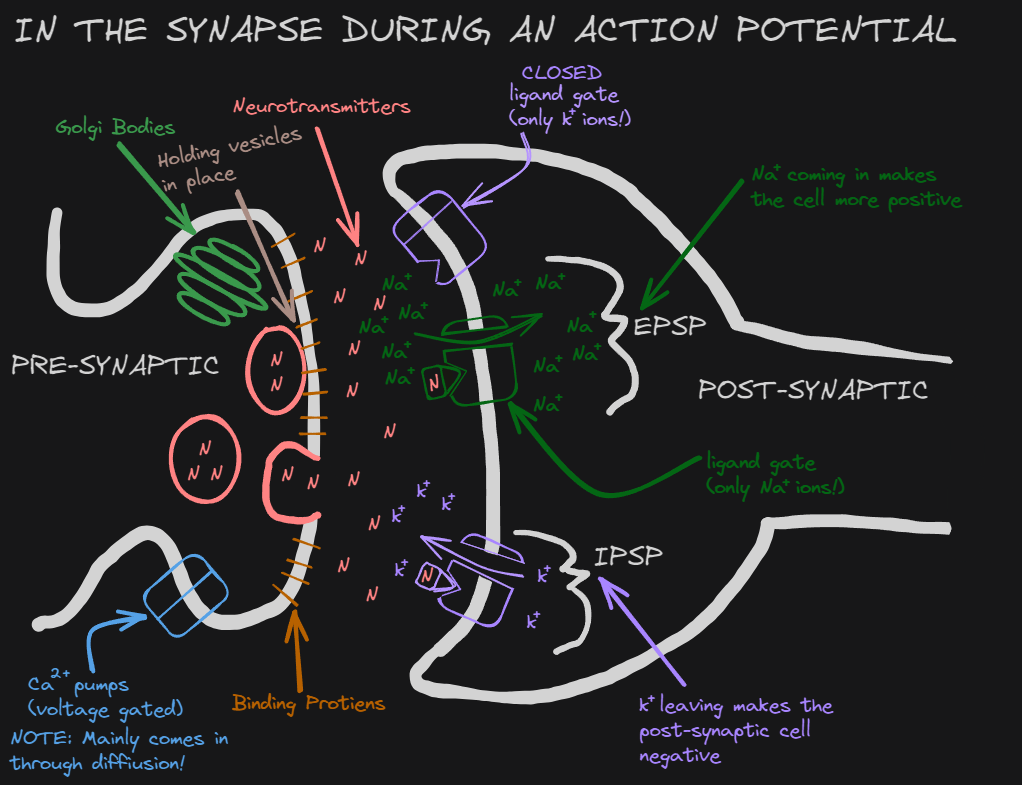
\includegraphics[width=.95\paperwidth,height=.95\paperheight,keepaspectratio]{excalidraw/neuron_synapse.png}
% \end{landscape}

% \begin{landscape}
%     \pagecolor{synapsebackground}
%     \pagestyle{plain}
%     \centering
%     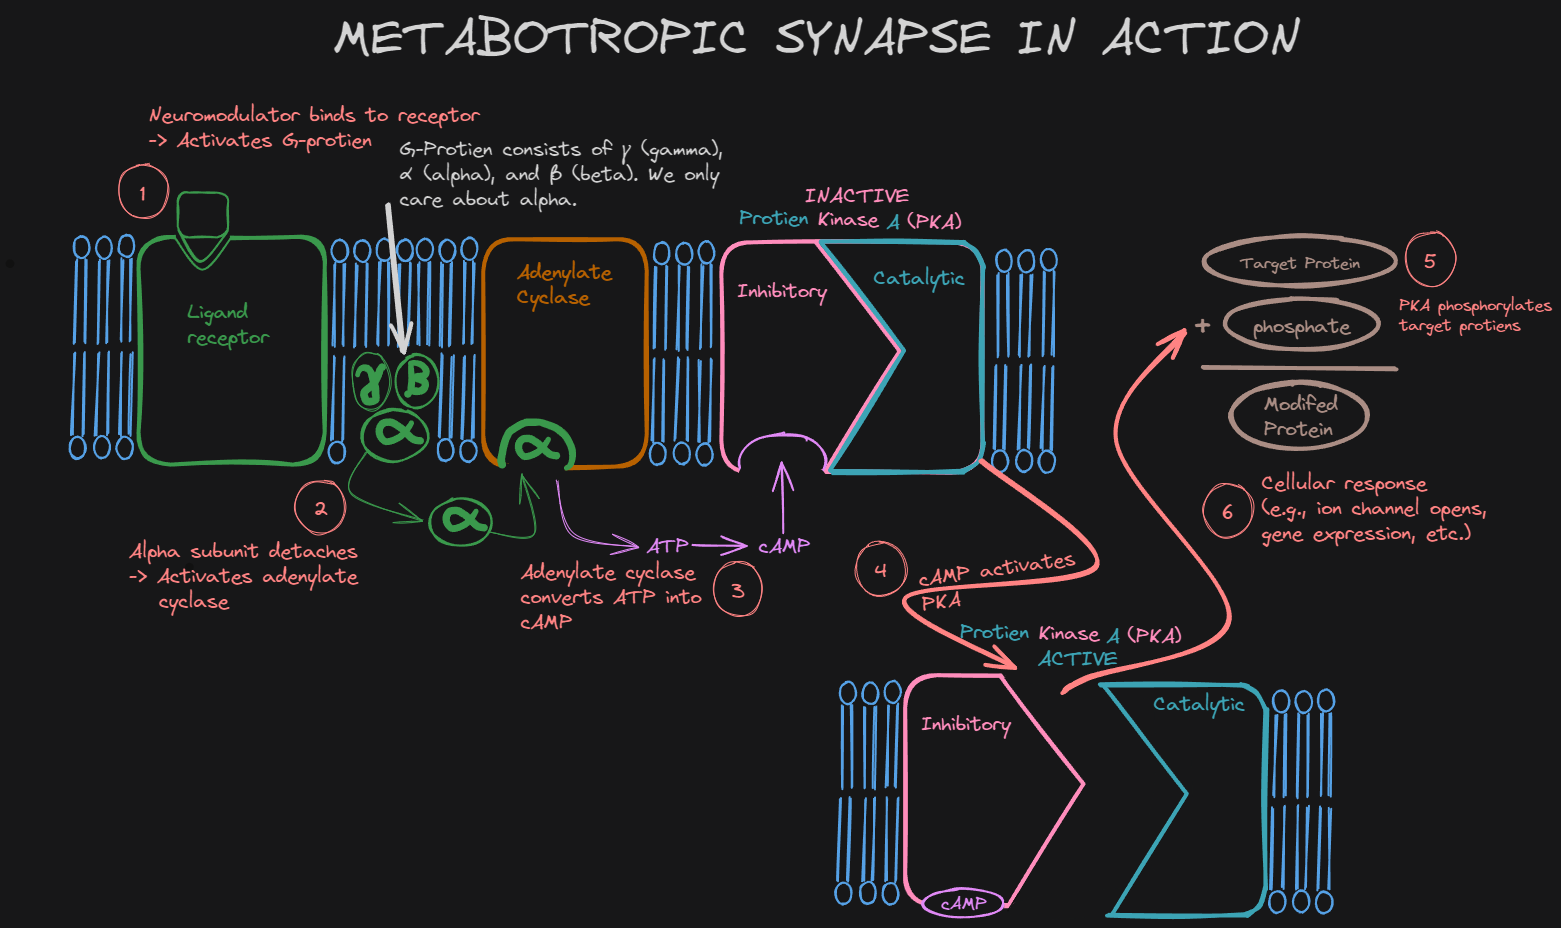
\includegraphics[width=.95\paperwidth,height=.95\paperheight,keepaspectratio]{excalidraw/metabotropic.png}
% \end{landscape}

% \pagecolor{draculabg}



\newpage
\begin{figure}[htbp]
    \centering
    \label{resting potential}
\begin{tikzpicture}
  % Labels for compartments
  \node at (-2,4.3) {\large \textbf{\underline{In}}};
  \node at (2,4.3) {\large \textbf{\underline{Out}}};
  \node at (-5.9,4.3) {\large \textbf{\underline{Permeability}}};

%   % Draw compartments as boxes
%   \draw (-5,-4) rectangle (-1,4); % Inside compartment
%   \draw (1,-4) rectangle (5,4);   % Outside compartment

  % Draw the membrane as a double line:
  % Left (solid) side denotes the negative (inside) and right (dotted) side the positive (outside)
  \draw[line width=1pt] (0.1,-4) -- (0.1,4);  
  \draw[dotted, line width=1pt] (-0.1,-4) -- (-0.1,4);

  % Place ion symbols on the "in" side (left) with relative sizes.
  % Here, potassium is large since it is more prevalent on the inside.
  \node (K_in) at (-3,2.5) {\huge \(\text{K}^{+}\)};
  \node (Na_in) at (-3,0) {\normalsize \(\text{Na}^{+}\)};
  \node (Cl_in) at (-3,-2.5) {\normalsize \(\text{Cl}^{-}\)};

  \node (P_K) at (-4.8,2.5) {\huge \(\text{P}\phantom{^{+}}\)};
  \node (P_K) at (-4.8,0) {\tiny \(\text{P}\phantom{^{+}}\)};
  \node (P_K) at (-4.8,-2.5) {\Large \(\text{P}\phantom{^{-}}\)};

  % Place ion symbols on the "out" side (right)
  % Here, sodium is made larger, etc.
  \node (K_out) at (3,2.5) {\normalsize \(\text{K}^{+}\)};
  \node (Na_out) at (3,0) {\huge \(\text{Na}^{+}\)};
  \node (Cl_out) at (3,-2.5) {\Large \(\text{Cl}^{-}\)};

  % Create nodes on the membrane for arrow connections
  \node (mem2_left) at (-0.5,0) {};
  \node (mem3_left) at (1.5,-2.5) {};
  \node (mem3_right) at (-1.5,-2.5) {};

  % Define arrow styles:
  \tikzset{
    diffusion/.style={->, >=Stealth, line width = 2pt, red},
    electric/.style={->, >=Stealth, line width = 2pt, blue}
  };

  % For each ion on the inside, draw two arrows (curved differently) going from the ion to the membrane.
  % The differences in the bending (and thus length) illustrate different magnitudes.
  % --- For K_in:
  \draw[electric, bend right=15] (K_in) to (K_out);
  \draw[diffusion, bend right=15, line width = 6pt] (K_out) to (K_in);
  % --- For Na_in:
  \draw[electric, bend left=15] (Na_out) to (mem2_left);
  \draw[diffusion, bend right=15] (Na_out) to (mem2_left);
  % --- For Cl_in:
  \draw[electric, bend right=15] (Cl_in) to (mem3_left);
  \draw[diffusion, bend right=15] (Cl_out) to (mem3_right);

  % Add a legend (key) to denote arrow styles.
  \node[draw, rectangle, right=1cm of K_out] (legend) {
    \begin{tabular}{ll}
      \textbf{Key:} & \\
      \tikz{\draw[diffusion, ->, >=Stealth, thick, red] (0,0) -- (1,0);} & Diffusion \\
      \tikz{\draw[electric, ->, >=Stealth, thick, blue] (0,0) -- (1,0);} & Electric \\
    \end{tabular}
  };
\end{tikzpicture}
\caption{The Resting Membrane Potential (RMP) of a Neuron}
\end{figure}

\begin{figure}[htbp]
    \centering
    \label{action potential}
\begin{tikzpicture}[scale=1.2]

    % Draw axes
    \draw[->, thick] (0,-4) -- (7,-4) node[right] {Time (ms)};
    \draw[->, thick] (0,-4) -- (0,3) node[above] {Voltage (mV)};

    % Draw threshold line at -55 mV and resting potential at -70 mV
    \draw[dashed] (0,-2.5) -- (7,-2.5) node[right] {Threshold (-55 mV)};
    \draw[dashed] (0,-3.5) -- (7,-3.5) node[right] {RMP (-70 mV)};
  
    % y-axis ticks and labels (scaling: 1 unit = 20 mV)
    \foreach \y/\label in {-3.5/{-70},-2.5/{-55}, -2/{-40}, -1/{-20}, 0/{0}, 1/{20}, 2/{40}} {
        \draw (0,\y) -- (-0.2,\y) node[left] {\label};
    }
    
    % x-axis ticks
    \foreach \x in {0,1,2,3,4,5,6} {
        \draw (\x,-4) -- (\x,-4.15) node[below] {\x};
    }
    
    % Draw action potential waveform using coordinates:
    % Points (x, y) where y = mV/20:
    % (0,-3.5):   Rest (-70 mV)
    % (1,-3.5):   Rest
    % (2,-2.75):  Threshold (-55 mV, since -55/20 = -2.75)
    % (3,2):      Peak depolarization (+40 mV, 40/20 = 2)
    % (4,-0.5):   Repolarization (-10 mV, -10/20 = -0.5)
    % (5,-4):     Hyperpolarization (-80 mV, -80/20 = -4)
    % (6,-3.5):   Return to rest (-70 mV)
    \draw[thick, horange] plot coordinates {
        (0,-3.5)
        (1,-3.5)
        (1.5,-3.5)
    };
    \draw[thick, horange, smooth] plot coordinates {
        (1.5,-3.5)
        (1.90,-2.55)
    };
    \draw[thick, horange] plot coordinates {
        (1.90,-2.55)
        (2,-2.5)
    };
    \draw[thick, horange, smooth] plot coordinates {
      (2,-2.5)
      (3,2)
      (4,-0.5)
      (5,-3.55)
      (6,-3.5)
    };

    % Add phase labels near the waveform
    \tikzset{
        circ/.style = {draw, circle, scale=0.7}
    };
    % Resting potential.
    \node[circ] at (1.3,-3.2) {1};
    % Opens sodium channels.
    \node[circ] at (1.75,-2.2) {2};
    % Potassium channels open.
    \node[circ] at (2.5,1.5) {3};
    % Sodium channels close.
    \node[circ] at (3.2,2.3) {4};
    % Potassium channels close.
    % \node[circ] at (6.1,-3.75) {5};
    
    \draw[decorate, decoration={brace, amplitude=5.5pt}]
    (5,-3.5) -- (6,-3.5);
    % Add text labels for phases
    \node at (2.2, 0) [rotate=78] {\textbf{Depolarization}};
    % The potassium is leaving the cell.
    \node at (4.2, 0) [rotate=287] {\textbf{Repolarization}};
    \node at (5.4, -3.1) {\textbf{Hyperpolarization}};

    % Arrow pointing hyperpolarization to -80 mv
    % \draw[->, thick] (7, -2) -- (4.93,-3.9) node[below] {};
  
  \end{tikzpicture}
    \caption{Action Potential Waveform}
\end{figure}



% \chapter*{Lab Practical 1}
% \addcontentsline{toc}{chapter}{Lab Practical 1}
% \vspace*{-0.25in}
% \section*{External Surface Structures}
\begin{itemize}
    \item \cyanit{Ansate Sulcus / Cruciate Fissure} - Located on the dorsal surface, separating frontal and parietal lobes.
    \item \cyanit{Medial Longitudinal Fissure} - Runs along the midline, separating the two cerebral hemispheres.
    \item \cyanit{Cerebellum} - Located at the posterior base of the brain.
    \item \cyanit{Coronal Sulcus / Superior Frontal Sulcus} - Found on the dorsal aspect, part of the frontal lobe.
    \item \cyanit{Transverse Fissure} - Separates the cerebellum from the cerebrum.
    \item \cyanit{Anterior / Rostral} - Toward the front of the brain.
    \item \cyanit{Posterior / Caudal} - Toward the back of the brain.
    \item \cyanit{Medial} - Toward the midline of the brain.
    \item \cyanit{Lateral} - Away from the midline.
\end{itemize}

\section*{Ventral Structures}
\begin{itemize}
    \item \cyanit{Olfactory Bulb} - Located at the most anterior portion of the ventral side.
    \item \cyanit{Cerebral Peduncle} - Found on the ventral midbrain, connects the cerebrum to the brainstem.
    \item \cyanit{Pons} - Bulging structure on the brainstem, anterior to the medulla.
    \item \cyanit{Pyramids on the Medulla} - Located on the ventral surface of the medulla oblongata.
    \item \cyanit{Spinal Cord} - Extends from the medulla caudally.
    \item \cyanit{Optic Chiasm} - X-shaped structure where optic nerves partially cross.
    \item \cyanit{Median Eminence / Tuber Cinereum} - Located at the base of the hypothalamus.
    \item \cyanit{Mammillary Body} - Small round structures part of the limbic system, posterior to the hypothalamus.
    \item \cyanit{Periamygdaloid Cortex / Uncus} - Located in the medial temporal lobe, part of the piriform cortex.
    \item \cyanit{Entorhinal Cortex} - Medial portion of the temporal lobe, key in memory processing.
    \item \cyanit{Lateral Olfactory Tract} - Extends from the olfactory bulb along the ventral surface.
    \item \cyanit{Rhinal Fissure} - Separates the neocortex from the piriform cortex.
    \item \cyanit{Insula / Island of Reil} - Located deep within the lateral sulcus.
    \item \cyanit{Sylvian Fissure} - Separates the temporal lobe from the frontal and parietal lobes.
\end{itemize}

\section*{Midbrain and Hindbrain Structures}
\begin{itemize}
    \item \cyanit{Superior Colliculus} - Dorsal midbrain, involved in visual processing.
    \item \cyanit{Inferior Colliculus} - Below the superior colliculus, involved in auditory processing.
    \item \cyanit{Pineal Body} - Small endocrine gland, located dorsally near the thalamus.
    \item \cyanit{Hypothalamus} - Located below the thalamus, controls endocrine functions.
    \item \cyanit{Corpus Callosum} - Large fiber bundle connecting the two cerebral hemispheres.
    \item \cyanit{Cingulate Gyrus} - Located superior to the corpus callosum, involved in emotion regulation.
    \item \cyanit{Cerebral Aqueduct} - Connects the third and fourth ventricles, running through the midbrain.
    \item \cyanit{Tegmentum} - Ventral part of the midbrain, involved in motor control.
    \item \cyanit{Massa Intermedia of the Thalamus} - Connects the two halves of the thalamus.
    \item \cyanit{Fornix} - White matter tract connecting the hippocampus to the hypothalamus.
\end{itemize}

\section*{Limbic System and Deep Brain Structures}
\begin{itemize}
    \item \cyanit{Hippocampus} - Located in the medial temporal lobe, essential for memory formation.
    \item \cyanit{Amygdala} - Anterior to the hippocampus, involved in emotion processing.
    \item \cyanit{Fimbria} - White matter tract leading from the hippocampus.
    \item \cyanit{Caudate Nucleus} - Part of the basal ganglia, involved in motor control.
    \item \cyanit{Lateral Ventricle} - Space within the corpus callosum, part of the ventricular system.
    \item \cyanit{Third Ventricle} - Space located between the two halves of the diencephalon.
\end{itemize}

% \begin{landscape}
%     \pagestyle{plain}
%     % \pagecolor{brainbackground}
%     \centering
%     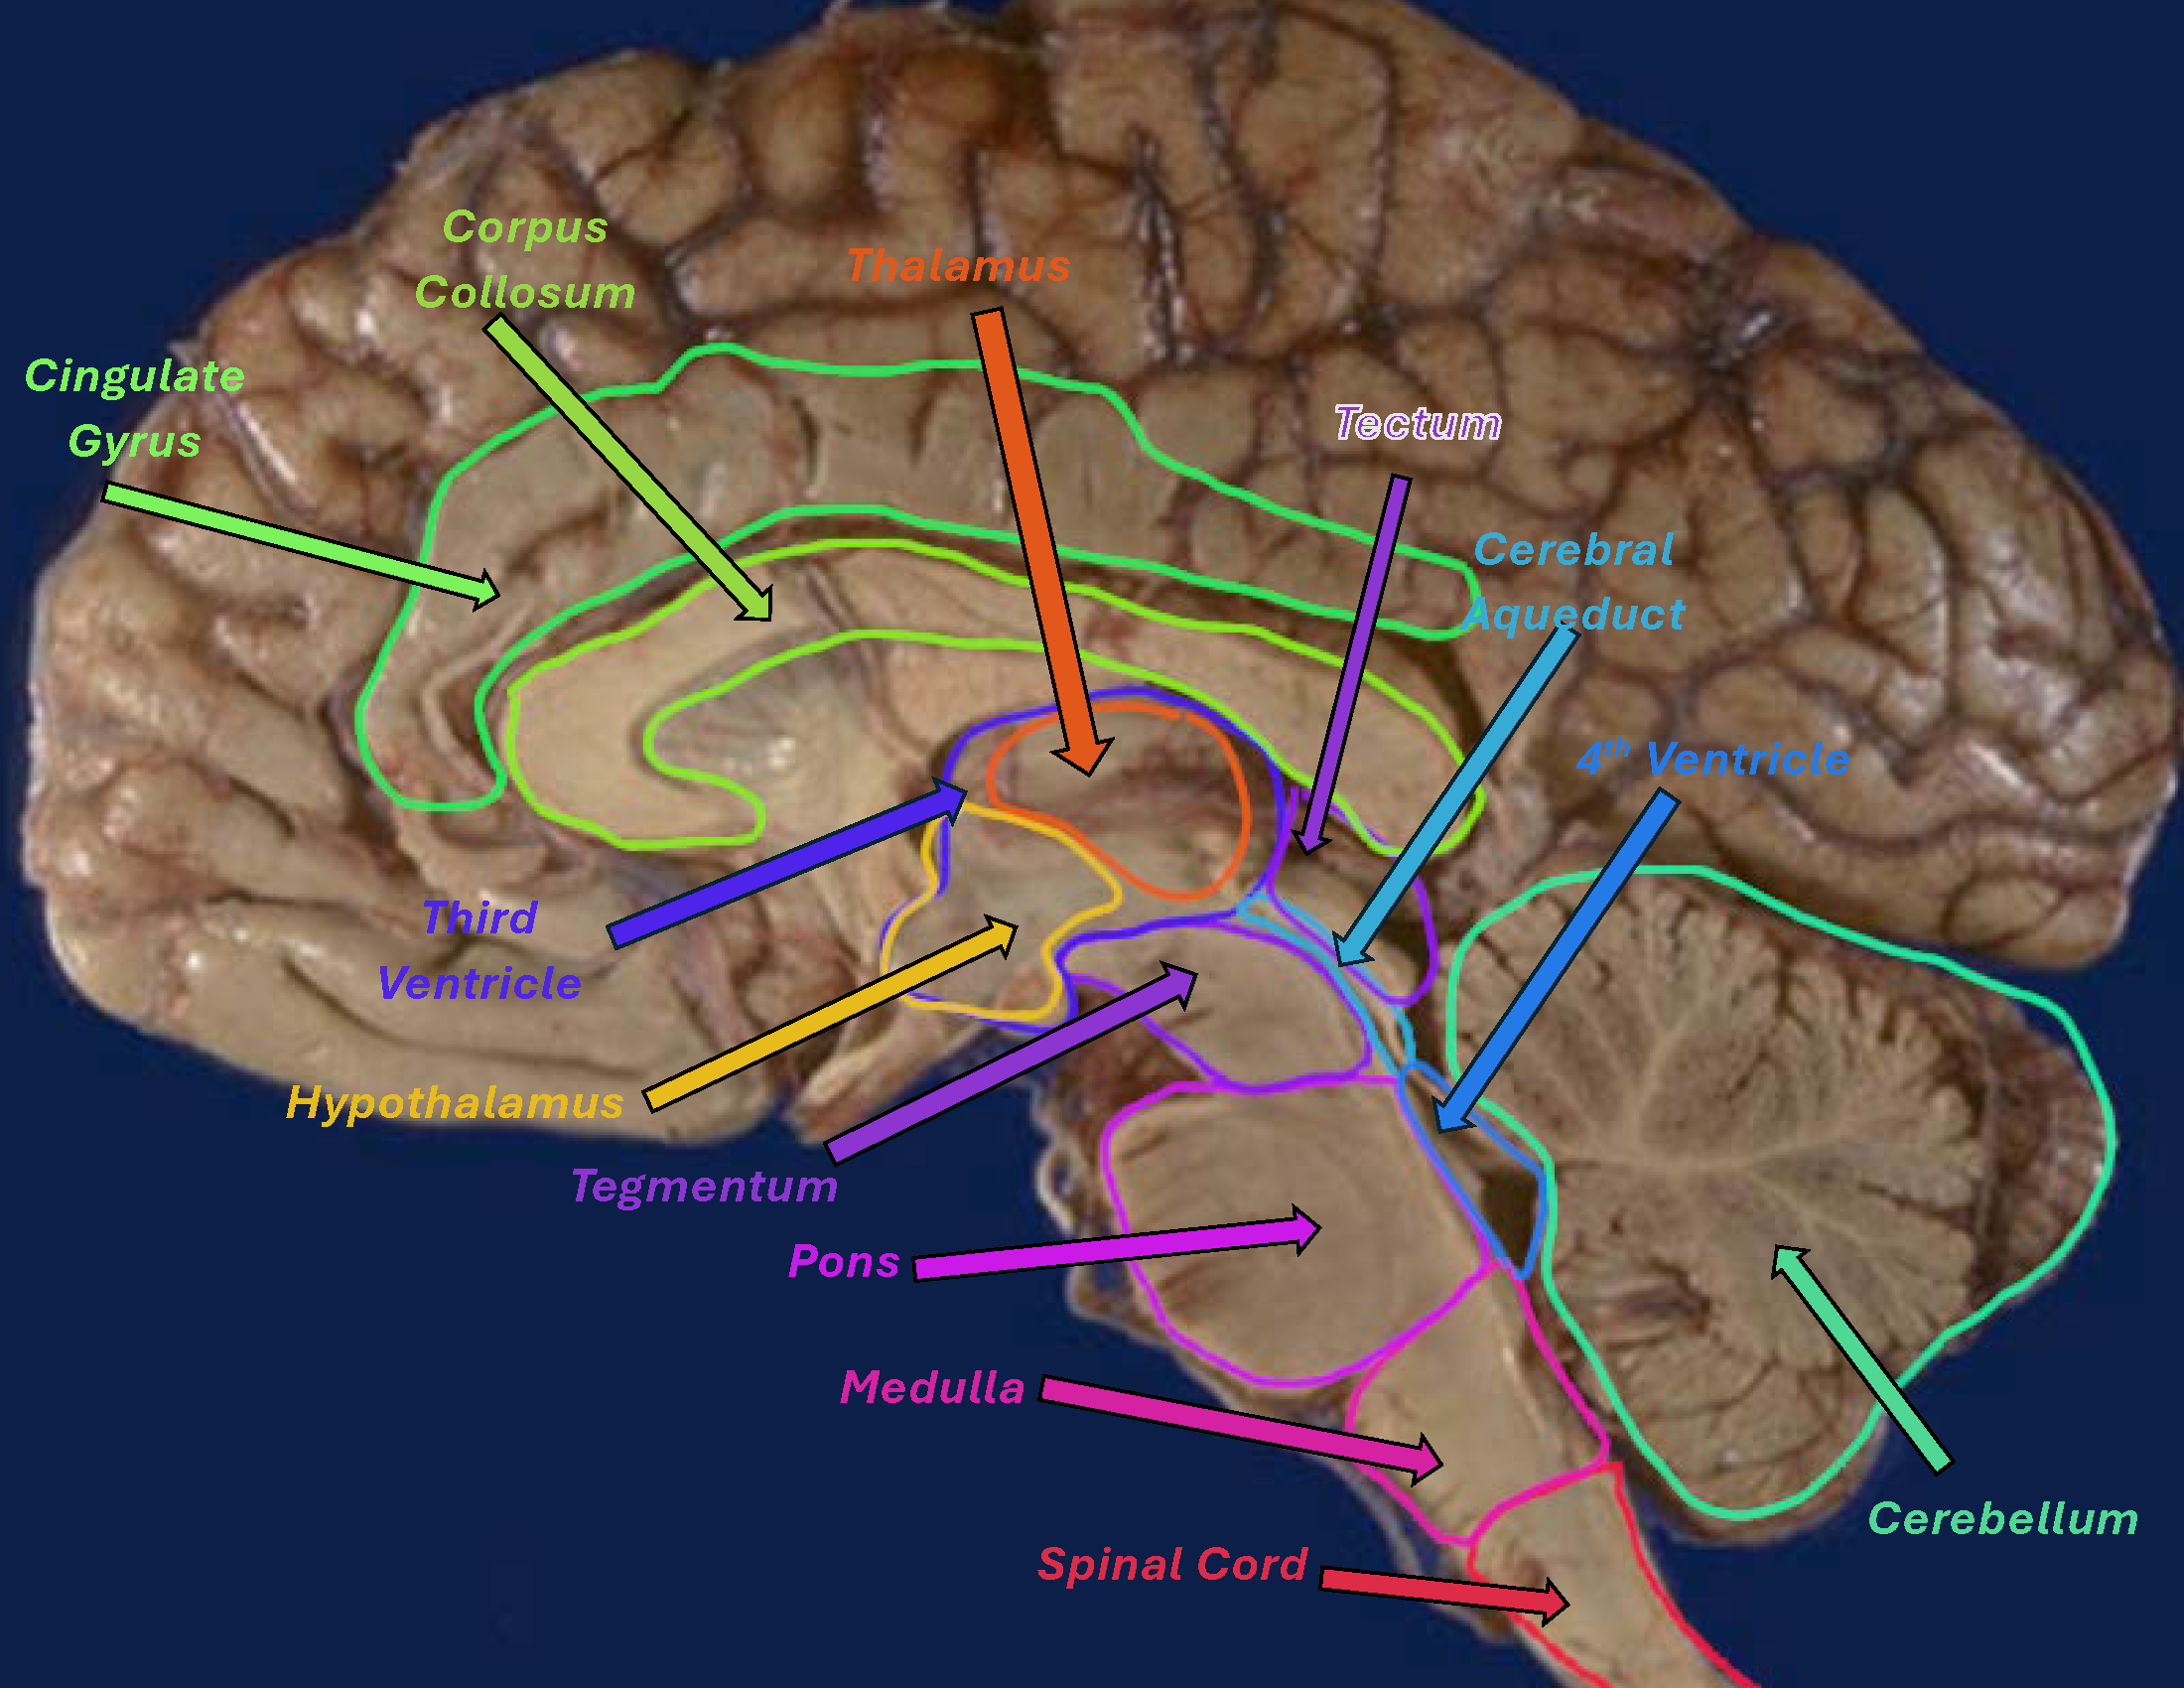
\includegraphics[width=.95\paperwidth,height=.95\paperheight,keepaspectratio]{images/midsagital_labeled.png}
%   \end{landscape}

% \chapter*{Exam 1b}
% \fancyhead[R]{Exam 1b}
% \addcontentsline{toc}{chapter}{Exam 1b}
% \vspace*{-0.25in}
% % ===========================
% Section 1.1: Neuroanatomy \& Nervous System Structure
% ===========================
\section*{1.1 \squigglyline}

\textbf{Directions:} For short answer questions, write your response in the space provided. Most of the short answer questions should be only a sentence or two long. For multiple choice questions, circle the letter of the correct response. For fill-in-the-blank questions, write your response in the space provided. For matching questions, write the letter of the correct response in the space to the right. For true or false questions, write ``True'' if the statement is true, and if the statement is false, \textit{explain why} the statement is false. Lastly, the sections (1.1, 1.2, etc.) are provided to break the exam into smaller parts. Good luck!

\begin{enumerate}[label=\textbf{Q1.1.\arabic*}]
      % Short answer question
      \item \textbf{Short Answer:} Define neuroscience. \\
            \textit{Answer:} \\%The study of the nervous system.

            % T/F question
      \item \textbf{True or False:} Behavioral neuroscience involves understanding the nervous system’s underlying behavior. \\
            \textit{Answer:} %True.

% Change this question
            % Fill in the blank
      \item \textbf{Fill in the Blank:} The Central Nervous System (CNS) is composed of the \underline{\hspace{2cm}} and the \underline{\hspace{2cm}}.
            \\
            %\textit{Answer:} Brain; spinal cord.

            % Matching question
      \item \textbf{Matching:} Match the following systems with their primary functions.
            \begin{wordbox}
                  \begin{enumerate}[label=(\roman*)]
                        \item Voluntary motor control and sensory input.
                        \item Involuntary control of the gastrointestinal system.
                        \item Involuntary control of smooth muscle and glands.
                  \end{enumerate}
            \end{wordbox}
            \begin{enumerate}[label=(\alph*)]
                  \item Somatic Nervous System \quad \dotfill \quad \underline{\hspace{3cm}}\\[0.5em]
                  \item Autonomic Nervous System \quad \dotfill \quad \underline{\hspace{3cm}}\\[0.5em]
                  \item Enteric Nervous System \quad \dotfill \quad \underline{\hspace{3cm}}
            \end{enumerate}
            %\textit{Answer:} (a) Voluntary motor control and sensory input; (b) Involuntary control of smooth muscle and glands; (c) Involuntary control of the gastrointestinal system.

% Change this question
      \item \textbf{Fill in the Blank} The autonomic nervous system regulates the body's \underline{\hspace{3cm}} AND \underline{\hspace{3cm}} response. \\
            %\textit{Answer} Fight or flight; rest and digest. OR Sympathetic; parasympathetic.

% Change this question
      \item \textbf{Short Answer:} How does the flight-or-flight response affect your body? \\
            \textit{Answer:} \\%Increases Heart rate, blood pressure, respiration, and alertness.

% Change this question
      \item \textbf{Fill in the Blank:} In the fecal microbiota transplant study, researchers found that the microbiota change the \underline{\hspace{3cm}} of the mice. \\
            %\textit{Answer:} Behavior.

% Change this question
      \item \textbf{Fill in the Blank:} In the elevated plus maze study, researchers found that the anxious mice were more willing to \underline{\hspace{3cm}} after the fecal microbiota transplant. \\
            %\textit{Answer:} Walk on the open arms.
\end{enumerate}

% ===========================
% Section 1.2: Meninges
% ===========================
\section*{1.2 \squigglyline}
\begin{enumerate}[label=\textbf{Q1.2.\arabic*}]
      \item \textbf{Short Answer:} What is the primary function of the meninges? \\
            \textit{Answer:} \\%To cover and protect the nervous system.

      \item \textbf{Multiple Choice:} Which of the following is the middle meningeal layer?
            \begin{tasks}[label=(\Alph*), label-width=1.5em, item-indent=1.7em](2) % two columns 
                  \task Arachnoid Membrane
                  \task Dura Mater
                  \task Pia Mater
                  \task Subarachnoid Space
            \end{tasks}
            %\textit{Answer:} A.

% Change this question. This is too easy.
      \item \textbf{Short Answer:} Why did early anatomists call the outermost meningeal layer ``pachymenginges''? \\
            \textit{Answer:} \\%Because it was similar to elephant skin.

      \item \textbf{Fill in the Blank} The Peripheral Nervous System uses \underline{\hspace{3cm}} layer(s) of the meninges. \\
            %\textit{Answer:} Two.

      \item \textbf{Fill in the Blank:} Arachnoid \underline{\hspace{3cm}} are web-like structures that connect the Arachnoid Membrane to the \textit{pia mater}
            %\textit{Answer:} trabeculae.

% Change this question
      \item \textbf{Fill in the Blank:} The subarachnoid space is filled with \underline{\hspace{3cm}}. \\
            %\textit{Answer:} Cerebrospinal fluid.

      \item \textbf{Short Answer:} What is meningitis? \\
            \textit{Answer:} \\%Inflammation of the meninges.

% Change this question
      % Changed question: Making the question more challenging by evaluating symptom combinations.
      \item \textbf{Multiple Choice:} Which combination of symptoms is LEAST consistent with a diagnosis of acute bacterial meningitis?
            \begin{tasks}[label=(\Alph*), label-width=1.5em, item-indent=1.7em](2)
                  \task Fever, headache, and nuchal rigidity.
                  \task Photophobia, vomiting, and altered mental status.
                  \task None of the above
            \end{tasks}
            %\textit{Answer:} D.
\end{enumerate}

% ===========================
% Section 1.3: Cerebrospinal Fluid (CSF)
% ===========================
\section*{1.3 \squigglyline}
\begin{enumerate}[label=\textbf{Q1.3.\arabic*}]
      \item \textbf{Short Answer:} List two functions of CSF. \\
            \textit{Answer:} \\%Protection, transportation of neurotransmitters, waste, hormones, and nutrients.

% Change this question
      \item \textbf{True or False:} CSF is similar in composition to blood plasma. \\
            \textit{Answer:} %True.

      \item \textbf{Fill in the Blank:} CSF is produced by the \underline{\hspace{3cm}} cells lining the lateral ventricles.
            %\textit{Answer:} ependymal.

      \item \textbf{Fill in the Blank:} A contra-coup injury is an injury that occurs on the \underline{\hspace{3cm}} side of the brain from the impact site.
            %\textit{Answer:} opposite.
\end{enumerate}

% ===========================
% Section 1.4: Flow of CSF
% ===========================
\section*{1.4 \squigglyline}
\begin{enumerate}[label=\textbf{Q1.4.\arabic*}]
      \item \textbf{Matching:} Match the location with its description.
            \begin{wordbox}
                  \begin{enumerate}[label=(\roman*)]
                        \item Connected to the pituitary gland via the infundibulum.
                        \item Production of CSF and connection to the third ventricle via the interventricular foramen.
                        \item Connects the third and fourth ventricles.
                  \end{enumerate}
            \end{wordbox}
            \begin{enumerate}[label=(\alph*)]
                  \item Lateral Ventricles \quad \dotfill \quad \underline{\hspace{3cm}}\\[0.5em]
                  \item Third Ventricle \quad \dotfill \quad \underline{\hspace{3cm}}\\[0.5em]
                  \item Cerebral Aqueduct \quad \dotfill \quad \underline{\hspace{3cm}}
            \end{enumerate}
            %\textit{Answer:} (a) Production of CSF and connection to the third ventricle via the interventricular foramen; (b) Connected to the pituitary gland via the infundibulum; (c) Connects the third and fourth ventricles.

      \item \textbf{True or False:} The central canal connects the fourth ventricle to the spinal cord. \\
            \textit{Answer:} %True.
\end{enumerate}

% ===========================
% Section 1.5: Dumping of CSF
% ===========================
\section*{1.5 \squigglyline}
\begin{enumerate}[label=\textbf{Q1.5.\arabic*}]
      \item \textbf{Short Answer:} Where is CSF absorbed into the bloodstream? \\
            \textit{Answer:} \\%Through the arachnoid villi/granulations into the superior sagittal sinus.

      \item \textbf{Fill in the Blank:} \underline{\hspace{3cm}} is caused by swelling of the brain due to a blockage in the CSF flow. \\
            %\textit{Answer:} Hydrocephalus.

% Change this question to a fill in the blank or multiple choice.
      \item \textbf{True or False:} The \textit{Interventricular Foramen} connects the lateral ventricles to the third ventricle. \\
            \textit{Answer:} %True.
\end{enumerate}

% ===========================
% Section 1.6: Getting Some CSF Out -- or -- Putting Something Into It
% ===========================
\section*{1.6 \squigglyline}

\begin{enumerate}[label=\textbf{Q1.6.\arabic*}]
      
% Change this question
      \item \textbf{Fill in the Blank:} The term ``\textit{epi}'' means \underline{\hspace{3cm}} and the term ``\textit{tap}'' means \underline{\hspace{3cm}}. \\
            %\textit{Answer:} %Something in; Taking something out.

      \item \textbf{Multiple Choice:} A lumbar puncture is sometimes called a:
            \begin{tasks}[label=(\Alph*), label-width=1.5em, item-indent=1.7em](2) % two columns 
                  \task Brain Tap
                  \task Spinal Tap
                  \task CSF Drain
                  \task Ventricular Tap
            \end{tasks}
            %\textit{Answer:} %B.

      \item \textbf{Fill in the Blank:} The needle for a lumbar puncture is typically inserted into the \underline{\hspace{3cm}} sac in the lumbar region.
            \\
            %\textit{Answer:} dural.
\end{enumerate}

% ===========================
% Section 1.7: Cranial Nerves
% ===========================
\section*{1.7 \squigglyline}
\begin{enumerate}[label=\textbf{Q1.7.\arabic*}]

      \item \textbf{Matching:} Match the cranial nerve number with its function.
            \begin{wordbox}
                  \begin{enumerate}[label=(\roman*)]
                        \item Facial sensation or motor control of the mandible
                        \item Vision
                        \item Smell
                  \end{enumerate}
            \end{wordbox}
            \begin{enumerate}[label=(\alph*)]
                  \item I \quad \dotfill \quad \underline{\hspace{3cm}}\\[0.5em]
                  \item II \quad \dotfill \quad \underline{\hspace{3cm}}\\[0.5em]
                  \item V \quad \dotfill \quad \underline{\hspace{3cm}}
            \end{enumerate}
            %\textit{Answer:} (a) Olfaction (smell); (b) Vision; (c) Facial sensation or motor control of the mandible.

      \item \textbf{True or False:} Cranial nerve IV controls pupil constriction and eye movement. \\
            \textit{Answer:} %False. (It only controls eye movement. OR, the statement is true if you're talking about cranial nerve III.)

      \item \textbf{Short Answer:} What is the function of cranial nerve X? \\
            \textit{Answer:} \\ %Taste and sensation from neck, thorax, abdomen, swallowing, control of laryx, parasympathetic nerves to heart and viscera.

% Change this question
      \item \textbf{Fill in the Blank:} There are \underline{\hspace{3cm}} cranial nerve(s) that modulate eye movements, and \underline{\hspace{3cm}} cranial nerve(s) that control the sense of vision. \\
            %\textit{Answer:} %Three; one.

      \item \textbf{True or False:} The term ``\textit{glossal}'' means ``taste''. \\
            \textit{Answer:} %False. (It means tongue.)

      \item \textbf{Fill in the Blank:} For the following table, fill in the blanks with the correct name.

% Add in sensory or motor or both column.
            \begin{multicols}{2}
                  \begin{tabular}{cc}
                        \toprule
                        \textbf{Cranial Nerve} & \textbf{Name}            \\ \midrule
                        I                      & \underline{\hspace{3cm}} \\[0.5em]
                        II                     & \underline{\hspace{3cm}} \\[0.5em]
                        III                    & \underline{\hspace{3cm}} \\[0.5em]
                        IV                     & \underline{\hspace{3cm}} \\[0.5em]
                        V                      & \underline{\hspace{3cm}} \\[0.5em]
                        VI                     & \underline{\hspace{3cm}} \\[0.5em]
                        \bottomrule
                  \end{tabular}
                  \begin{tabular}{cc}
                        \toprule
                        \textbf{Cranial Nerve} & \textbf{Name}            \\ \midrule
                        VII                    & \underline{\hspace{3cm}} \\[0.5em]
                        VIII                   & \underline{\hspace{3cm}} \\[0.5em]
                        IX                     & \underline{\hspace{3cm}} \\[0.5em]
                        X                      & \underline{\hspace{3cm}} \\[0.5em]
                        XI                     & \underline{\hspace{3cm}} \\[0.5em]
                        XII                    & \underline{\hspace{3cm}} \\[0.5em]
                        \bottomrule
                  \end{tabular}
            \end{multicols}

\end{enumerate}

% ===========================
% Section 1.8: Terms
% ===========================
\section*{1.8 \squigglyline}
\begin{enumerate}[label=\textbf{Q1.8.\arabic*}]

      \item \textbf{Short Answer:} What does the term \textit{Soma} refer to? \\
            \textit{Answer:}% The cell body of a neuron.

      \item \textbf{True or False:} The term ``\textit{nucleus}'' refers to a collection of cell bodies in the PNS. \\
            \textit{Answer:} %False. (It refers to a collection of cell bodies in the CNS.)

      \item \textbf{Fill in the Blank:} Fill in the following table for the terms that match its definition. \\

            \begin{tabular}[htbp]{cc}
                  \toprule
                  \textbf{Term}            & \textbf{Definition}                           \\ \midrule
                  Tract                    & \underline{\hspace{10cm}}                     \\[0.5em]
                  \underline{\hspace{3cm}} & The ends of the neuron that send information. \\[0.5em]
                  \underline{\hspace{3cm}} & Extends surface area of the neuron.           \\[0.5em]
                  \underline{\hspace{3cm}} & A collection of axons in the PNS.             \\        \bottomrule
            \end{tabular}
            %\textit{Answer:} %A collection of axons in the CNS; axonal buttons; dendrites; nerve.

      \item \textbf{True or False:} \textit{Ganglion} are collections of axons. \\
            \textit{Answer:} %False. (They are collections of cell bodies.)

      \item \textbf{Short Answer:} What is the function of the myelin sheath? \\
            \textit{Answer:} %To insulate the axon and speed up the transmission of the action potential.
\end{enumerate}

% ===========================
% Section 1.9: Brainstem --- Hindbrain and Midbrain
% ===========================
\section*{1.9 \squigglyline}
\begin{enumerate}[label=\textbf{Q1.9.\arabic*}]
      \item \textbf{Short Answer:} Name two principal structures of the hindbrain. \\
            \textit{Answer:} \\%Medulla Oblongata and Pons (or Cerebellum).

      \item \textbf{Short Answer:} What vital functions are regulated by the Reticular Formation in the Medulla Oblongata? \\
            \textit{Answer:} \\ % Heart rate, blood pressure, respiration.

      \item \textbf{Short Answer:} Describe the role of the Pons in the brainstem. \\
            \textit{Answer:} % Acts as a bridge connecting various brain regions and houses the Locus Coeruleus.

      \item \textbf{Fill in the Blank:} Pons directly translates to \underline{\hspace{3cm}} in Latin. \\
            %\textit{Answer:} %Bridge.

      \item \textbf{Fill in the Blank:} The \underline{\hspace{3cm}} (specific) is a structure in the pons that produces norepinephrine. \\
            %\textit{Answer:} %Locus Coeruleus.

% Change this question. It directly answers the question before it.
      \item \textbf{True or False:} The norepinephrine produced by the Locus Coeruleus is sent primarily to the hind brain. \\
            \textit{Answer:} %False. (It is sent to the forebrain.)

      \item \textbf{Short Answer:} What is the primary function of the cerebellum? \\
            \textit{Answer:} %Coordination of movement and balance.

      \item \textbf{\textit{Bonus} Short Answer:} Can you name every function of the cerebellum? (There's 8!) \\
            \textit{Answer:} \\[0.5em]%Balance, hand-eye coordination, soothes movements, shifts attention between vision and hearing, sensory timing (judging rhythm), language, emotional control, and reward valuation.

      \item \textbf{Fill in the Blank:} The rare malformation wherein the cerebellum is not developed is called \underline{\hspace{3cm}}. \\
            %\textit{Answer:} %Cerebellar agenesis.

% Change this question. It is answered by a later question.
      \item \textbf{Multiple Choice:} Which of the following midbrain structures is primarily responsible for visual reflexes? \\
            (A) Olives \quad (B) Pyramids \quad (C) Superior Colliculus \quad (D) Substantia Nigra \\
            %\textit{Answer:} %C.

      \item \textbf{Fill in the Blank:} The \underline{\hspace{3cm}} in the midbrain is critical for motor coordination. \\
            %\textit{Answer:} %Red nucleus.

      \item \textbf{Short Answer:} What does the \textit{periaqueductal gray area} produce? \\
            \textit{Answer:} \\%Opioiods

% Change this question to fill in the blank.
      \item \textbf{True or False:} The medulla oblongata contains the reticular formation which regulates vital functions like heart rate and respiration. \\
            \textit{Answer:} %True.

% Change this question. It answers the question referenced before.
      \item \textbf{Fill in the Blank:} The midbrain’s \underline{\hspace{3cm}} Colliculus is important for visual reflexes, while the \underline{\hspace{3cm}} Colliculus is involved in auditory reflexes.
            % \textit{Answer:} Superior; Inferior.

      \item \textbf{Multiple Choice:} The \textit{substantia nigra} is known for its role in:
            \begin{enumerate}[label=(\Alph*)]
                  \item Serotonin production
                  \item Dopamine production
                  \item GABA production
                  \item Acetylcholine production
            \end{enumerate}
            %\textit{Answer:} %B.
\end{enumerate}

% ===========================
% Section 1.10: Forebrain --- Diencephalon and Telencephalon
% ===========================
\section*{1.10 \squigglyline}
\begin{enumerate}[label=\textbf{Q1.10.\arabic*}]
      \item \textbf{Short Answer:} What is the role of the thalamus in the brain? \\
            \textit{Answer:} %It relays sensory and motor signals

      \item \textbf{Fill in the Blank:} Fill in the following table with the correct terms.
            \begin{table}[htbp]
                  \centering
                  \begin{tabular}{cc}
                        \toprule
                        \textbf{Thalamic Relay Nuclei} & \textbf{Description} \\ \midrule
                        \underline{\hspace{3cm}}       & Vision               \\
                        \underline{\hspace{3cm}}       & Pain                 \\
                        \underline{\hspace{3cm}}       & Promotes wakefulness \\
                        \bottomrule
                  \end{tabular}
            \end{table}
            %\textit{Answer:} %Lateral Geniculate Nucleus; Dorsal Medial Nucleus; Nucleus Reticularis

% Change this question
      \item \textbf{Short Answer:} What does it mean to be a non-specific relay nuclei? \\
            \textit{Answer:} %It means that the thalamic nuclei do not have a specific function.

      \item \textbf{Multiple Choice:} The thalamic nucleus responsible for pain routing sends those signals to the:
            \begin{tasks}[label=(\Alph*), label-width=1.5em, item-indent=1.7em](2) % two columns 
                  \task Prefrontal Cortex
                  \task Primary Somatosensory Cortex
                  \task Primary Motor Cortex
                  \task Amygdala
            \end{tasks}
            %\textit{Answer:} %A.

% Either move this question to a different spot or change it.
      \item \textbf{Fill in the Blank:} The \textit{Massa Intermedia} connects the left \underline{\hspace{3cm}} half with the right half. \\
            %\textit{Answer:} %Thalamus.

      \item \textbf{Multiple Choice:} Which of the following is NOT a function of the hypothalamus?
            \begin{enumerate}[label=(\Alph*)]
                  \item Survival of the individual
                  \item Survival of the species
                  \item Regulation of endocrine system
                  \item Integration of information
            \end{enumerate}
            %\textit{Answer:} %C.



% Change this question
      \item \textbf{True or False:} The hypothalamus is involved in both individual survival functions (like eating and drinking) and species survival functions (such as reproduction). \\
            \textit{Answer:} %True.


% Change this question. Possibly multiple choice instead.
      \item \textbf{True or False:} The \textit{Suprachiasmatic Nucleus} is responsible for circadian rhythms. \\
            \textit{Answer:} %True.

% Change this question. Too easy with process of elimination.   
      \item \textbf{Matching:} Match the following telencephalic structures with their functions.
            \begin{wordbox}
                  \begin{enumerate}[label=(\roman*)]
                        \item Sensory integration and spatial awareness.
                        \item Executive functions, motor control, language production.
                        \item Memory, hearing, language comprehension.
                        \item Vision
                  \end{enumerate}
            \end{wordbox}
            \begin{enumerate}[label=(\alph*)]
                  \item Frontal Lobe \quad \dotfill \quad \underline{\hspace{3cm}}\\[0.5em]
                  \item Temporal Lobe \quad \dotfill \quad \underline{\hspace{3cm}}\\[0.5em]
                  \item Parietal Lobe \quad \dotfill \quad \underline{\hspace{3cm}}\\[0.5em]
                  \item Occipital Lobe \quad \dotfill \quad \underline{\hspace{3cm}}
            \end{enumerate}
            %\textit{Answer:} (a) Executive functions, motor control, language production; (b) Memory, hearing, language comprehension; (c) Sensory integration and spatial awareness. (d) Vision.

      \item \textbf{Fill in the Blank:} The \textit{Corpus Callosum}'s neurons go from \underline{\hspace{3cm}} to \underline{\hspace{3cm}} and not from \underline{\hspace{3cm}} to \underline{\hspace{3cm}}. (Your answers should directions.) \\
            %\textit{Answer:} %Lateral to lateral; dorsal to ventral.

      \item \textbf{Multiple Choice:} Which of the following is NOT a symptom of Callosal Agenesis?
            \begin{tasks}[label=(\Alph*), label-width=1.5em, item-indent=1.7em](2) % two columns 
                  \task Impaired motor coordination
                  \task Impaired language comprehension
                  \task Impaired spatial awareness
                  \task Impaired executive functions
            \end{tasks}
            %\textit{Answer:} %B.

      \item \textbf{Fill in the Blank:} The \underline{\hspace{3cm}} is involved in the regulation of voluntary motor control. \\
            %\textit{Answer:} %Basal Ganglia.

      \item \textbf{Fill in the Blank:} The \textit{Striatum} consists of the \underline{\hspace{3cm}}, \underline{\hspace{3cm}}, and the \underline{\hspace{3cm}}. (\textit{Note:} The \textit{Globus Pallidus} is not a viable answer here.) \\
            %\textit{Answer:} %Caudate Nucleus; Putamen, Nucleus accumbens.

      \item \textbf{True or False:} When people mention the Nucleus Accumbens and the Globus Pallidus, they call it the lentiform nucleus. \\
            \textit{Answer:} %False. (The putamen and the globus pallidus are called the lentiform nucleus.)

      \item \textbf{Fill in the Blank:} Participants in Rees et al.'s (2011) study showed extreme conservatives had a larger \underline{\hspace{3cm}} \\
            %\textit{Answer:} %Amygdala.

      \item \textbf{Short Answer:} How does the hippocampus have an impact upon memory? \\
            \textit{Answer:} %Moves memories from short-term to long-term storage.

      \item \textbf{Short Answer:} What is the left hemisphere of the brain responsible for? And the right hemisphere? (2 each.) \\
            \textit{Answer:} \\%Left: Language, serial events; Right: Creativity, synthesis of information. 

      \item \textbf{Matching:} Arrange the following structures in the brain in the right order.
      \begin{wordbox}
            \begin{enumerate}[label=(\roman*)]
                  \item Tectum
                  \item Medulla Oblogata
                  \item Limbic System
                  \item Hypothalamus
            \end{enumerate}
      \end{wordbox}
      \begin{enumerate}[label=(\alph*)]
            \item Myelencephalon \quad \dotfill \quad \underline{\hspace{3cm}}\\[0.5em]
            \item Diencephalon \quad \dotfill \quad \underline{\hspace{3cm}}\\[0.5em]
            \item Telencephalon \quad \dotfill \quad \underline{\hspace{3cm}}\\[0.5em]
            \item Mesencephalon \quad \dotfill \quad \underline{\hspace{3cm}}\\
      \end{enumerate}
      %\textit{Answer:} %B, D, C, A.

      \item \textbf{Short Answer:} What is \textit{Kluver-Bucy Syndrome}? \\
            \textit{Answer:} %A condition where the amygdala is damaged, leading to loss of normal fear and anger responses.

      \item \textbf{Fill in the Blank:} The \underline{\hspace{3cm}} is involved in the regulation of emotions, memory, and motivation. \\
            %\textit{Answer:} %Limbic System.

      \item \textbf{Fill in the Blank:} Selective attention, love, and pain are all functions of the \underline{\hspace{3cm}}. \\
            %\textit{Answer:} %Cingulate gyrus.

      \item \textbf{Short Answer:} What lobes make up the \textit{Cerebral Cortex}? \\
            \textit{Answer:} \\%Frontal, Parietal, Temporal, Occipital.

      \item \textbf{Short Answer:} We learned that the \textit{Temporal Lobe} is responsible for language comprehension. Who was the scientist that discovered this? Similarly, we learned that the \textit{Frontal Lobe} is responsible for language production. Who was the scientist that discovered this? \\
            \textit{Answer:} \\%Wernicke; Broca.

      \item \textbf{Multiple Choice:} In a study by Eisenberger (1990) called the Cyberball study, participants who were excluded from the game showed increased activity in the:
            \begin{tasks}[label=(\Alph*), label-width=1.5em, item-indent=1.7em](2) % two columns 
                  \task Amygdala
                  \task Hippocampus
                  \task Anterior Cingulate Cortex
                  \task Septal Nucleus
            \end{tasks}
            %\textit{Answer:} %C.

      \item \textbf{Fill in the Blank:} Fill out the following table with the correct terms.
\end{enumerate}

\begin{table}[ht]
      \centering
      \begin{tabular}{l l l l}
            \toprule
            \textbf{Major Divisions} & \textbf{Ventricle}                                       & \textbf{Subdivision}          & \textbf{Principal Structures} \\
            \midrule

            %--- Forebrain Block ----------------------------------
            \multirow{7}{*}{Forebrain}
                                     & \multirow{5}{*}{\underline{\hspace{3cm}}}
                                     & \multirow{4}{*}{\underline{\hspace{3cm}}}
                                     & \underline{\hspace{3cm}}                                                                                   \\
                                     &                                                          &
                                     & \underline{\hspace{3cm}}                                                                                   \\
                                     &                                                          &
                                     & \underline{\hspace{3cm}}                                                                                     \\
                                     &                                                          &
                                     & \underline{\hspace{3cm}}                                                                                     \\[0.5em]
            \cline{3-4}                                                                                                                                         \\[-0.5em]
                                     & \multirow{2}{*}{\underline{\hspace{3cm}}}             & \multirow{2}{*}{\underline{\hspace{3cm}}}
                                     & \underline{\hspace{3cm}}                                                                                          \\
                                     &                                                          &
                                     & \underline{\hspace{3cm}}                                                                                      \\
            \midrule

            %--- Midbrain Block ------------------------------------
            \multirow{4}{*}{Midbrain}
                                     & \multirow{4}{*}{\underline{\hspace{3cm}}}
                                     & \multirow{4}{*}{\underline{\hspace{3cm}}}
                                     & \underline{\hspace{3cm}}                                                                                             \\
                                     &                                                          &
                                     & \underline{\hspace{3cm}}                                                                                         \\
                                     &                                                          &
                                     & \underline{\hspace{3cm}}                                                                               \\
                                     &                                                          &
                                     & \underline{\hspace{3cm}}                                                                               \\
            \midrule

            %--- Hindbrain Block -----------------------------------
            \multirow{4}{*}{Hindbrain}
                                     & \multirow{4}{*}{\underline{\hspace{3cm}}}
                                     & \multirow{2}{*}{\underline{\hspace{3cm}}}
                                     & \underline{\hspace{3cm}}                                                                                        \\
                                     &                                                          &
                                     & \underline{\hspace{3cm}}                                                                                               \\[0.5em]
            \cline{3-4}                                                                                                                                         \\[-0.5em]
                                     &                                                          & \underline{\hspace{3cm}}
                                     & \underline{\hspace{3cm}}                                                                                 \\
            \bottomrule
      \end{tabular}
      \label{tab:brain-divisions}
\end{table}

% ===========================
% Section 1.11: Parkinson's and Alzheimer's Disease
% ===========================
\section*{1.11 \squigglyline}
\begin{enumerate}[label=\textbf{Q1.11.\arabic*}]
      \item \textbf{Multiple Choice:} Which of the following is NOT a typical symptom of Parkinson's Disease? \\
            (A) Bradykinesia \quad (B) Rigidity \quad (C) Tremors \quad (D) Hyperactivity
            %\textit{Answer:} %D

      \item \textbf{Short Answer:} Name one symptom associated with Alzheimer's Disease. \\
            \textit{Answer:} %Progressive memory loss.

      \item \textbf{True or False:} Only retrograde amnesia is observed in Alzheimer's Disease. \\
            \textit{Answer:} %False. (Both retrograde and anterograde amnesia are observed.)
\end{enumerate}


% \chapter*{Exam 2}
% \fancyhead[R]{Exam 2}
% \addcontentsline{toc}{chapter}{Exam 2}
% \vspace*{-0.25in}
% % ===========================
% Section 2.1 -- The Neuron
% ===========================
\section*{2.1}
\begin{enumerate}[label=\textbf{Q2.1.\arabic*}]
      \item \textbf{Short Answer:} Define a neuron. \\
            % \textit{Answer:} Basic information processing unit of the nervous system.
      \item \textbf{Multiple Choice:} Which cell type forms the myelin sheath in the CNS?
            \begin{tasks}[label=\textcolor{draculafg}{(\Alph*)}, item-format=\color{draculafg}, label-width=1.5em, item-indent=1.7em](2)
                  \task Oligodendrocytes
                  \task Schwann Cells
                  \task Astrocytes
                  \task Satellite Cells
            \end{tasks}
            % \textit{Answer:} A
      \item \textbf{Fill in the Blank:} The process by which glial cells remove debris is called \underline{\hspace{3cm}}. \\
            % \textit{Answer:} Phagocytosis.
      \item \textbf{Short Answer:} Name two functions of astrocytes. \\
            % \textit{Answer:} Provide structural support and deliver nutrients to neurons.
      \item \textbf{Fill in the Blank:} \underline{\hspace{3cm}} are responsible for myelination in the PNS. \\
            % \textit{Answer:} Schwann Cells.
      \item \textbf{Multiple Choice:} What is one function of myelin?
            \begin{tasks}[label=\textcolor{draculafg}{(\Alph*)}, item-format=\color{draculafg}, label-width=1.5em, item-indent=1.7em](2)
                  \task Insulate axons
                  \task Synthesize proteins
                  \task Produce neurotransmitters
                  \task Break down debris
            \end{tasks}
            % \textit{Answer:} A.
      \item \textbf{Fill in the Blank:} Glial cells compose about half of nervous tissue volume, but are approximately \underline{\hspace{3cm}} times more numerous than neurons. \\
            % \textit{Answer:} 10-50.

      \item \textbf{Short Answer:} What are two similarities between neurons and other animal cells? \\
            % \textit{Answer:} They have a cell membrane, a nucleus, and a variety of organelles.
      \item \textbf{Short Answer:} In neurons, what is the primary role of mitochondria? \\
            % \textit{Answer:} Producing energy for the cell.
      \item \textbf{Fill in the Blank:} The organelle responsible for protein synthesis in neurons is the \underline{\hspace{3cm}}. \\
            % \textit{Answer:} Endoplasmic Reticulum.
      \item \textbf{Fill in the Blank:} The \underline{\hspace{3cm}} packages neurotransmitters for transport. \\
            % \textit{Answer:} Golgi Apparatus.
      \item \textbf{Fill in the Blank:} Organelles that break down waste products in neurons are called \underline{\hspace{3cm}}. \\
            % \textit{Answer:} Lysosomes.
      \item \textbf{Short Answer:} What distinguishes the morphology of neurons from typical animal cells? \\
            % \textit{Answer:} Neurons have long processes (axons and dendrites) specialized for signal transmission.
      \item \textbf{Fill in the Blank:} Neurons communicate via an \underline{\hspace{3cm}} process. \\
            % \textit{Answer:} electrochemical.
      \item \textbf{Multiple Choice:} Which cell type is primarily responsible for debris removal in the CNS?
            \begin{tasks}[label=\textcolor{draculafg}{(\Alph*)}, item-format=\color{draculafg}, label-width=1.5em, item-indent=1.7em](2)
                  \task Microglia
                  \task Astrocytes
                  \task Oligodendrocytes
                  \task Satellite Cells
            \end{tasks}
            % \textit{Answer:} A.
      \item \textbf{Multiple Choice:} Which cells line the ventricles and help form CSF?
            \begin{tasks}[label=\textcolor{draculafg}{(\Alph*)}, item-format=\color{draculafg}, label-width=1.5em, item-indent=1.7em](2)
                  \task Astrocytes
                  \task Ependymal Glia
                  \task Schwann Cells
                  \task Microglia
            \end{tasks}
            % \textit{Answer:} B.
      \item \textbf{Short Answer:} What is the function of satellite cells in the PNS? \\
            % \textit{Answer:} They provide nutrients and physical support to neurons.

      \item \textbf{Multiple Choice:} Which glial cell in the PNS is notably associated with neuronal regeneration?
            \begin{tasks}[label=\textcolor{draculafg}{(\Alph*)}, item-format=\color{draculafg}, label-width=1.5em, item-indent=1.7em](2)
                  \task Oligodendrocytes
                  \task Microglia
                  \task Satellite Cells
                  \task Schwann Cells
            \end{tasks}
            % \textit{Answer:} D.

      \item \textbf{Multiple Choice:} What happens during maintenance of internal consistency?
            \begin{tasks}[label=\textcolor{draculafg}{(\Alph*)}, item-format=\color{draculafg}, label-width=1.5em, item-indent=1.7em](1)
                  \task Microglia remove cellular debris.
                  \task Oligodendrocytes myelinate axons.
                  \task Astrocytes absorb excess potassium ions.
                  \task Schwann cells provide nutrients to neurons.
            \end{tasks}
            % \textit{Answer:} C.
      \item \textbf{Long Answer:} What evidence supports the notion that glial cells' malfunctioning may be contributing to Alzheimer's Disease? (Your answer must include beta amyloid, Tau, and the possible cause of Alzheimer's Disease.) \\
            % \textit{Answer:} Glial cells normally remove beta amyloid plaques, but if it builds up too much outside the cell, Tau builds up inside the cell. This leads to inflammation, which may be the problem of Alzheimer's Disease.

\end{enumerate}
\newpage
\squigglyline
% ===========================
% Section 2.2 Different Kinds of Neurons
% ===========================

\section*{2.2}
\begin{enumerate}[label=\textbf{Q2.2.\arabic*}]

      \item \textbf{Fill in the Blank:} The three structural classifications of neurons are \underline{\hspace{3cm}}, \underline{\hspace{3cm}}, and \underline{\hspace{3cm}}. \\
            % \textit{Answer:} Unipolar; Bipolar; Multipolar.



      \item \textbf{Fill in the Blank:} Neurons are based on \underline{\hspace{3cm}} and \underline{\hspace{3cm}}. \\
            % \textit{Answer:} Structure; function.


      \item \textbf{Fill in the Blank:} Sensory neurons carry information from the \underline{\hspace{3cm}} to the \underline{\hspace{3cm}}. \\
            % \textit{Answer:} PNS; CNS.

      \item \textbf{Short Answer:} What is the primary function of motor neurons? \\
            % \textit{Answer:} To carry information from the CNS to muscles and glands.

      \item \textbf{Multiple Choice:} What does ``Efferent'' mean?
            \begin{tasks}[label=\textcolor{draculafg}{(\Alph*)}, item-format=\color{draculafg}, label-width=1.5em, item-indent=1.7em](4)
                  \task Incoming
                  \task Sensory
                  \task Motor
                  \task Outgoing
            \end{tasks}
            % \textit{Answer:} D.

\end{enumerate}
\squigglyline

% ===========================
% Section 2.3 Neural Communication
% ===========================

\section*{2.3}
\begin{enumerate}[label=\textbf{Q2.3.\arabic*}]


      \item \textbf{Short Answer:} What are the 2 systems of neuronal communication? \\
            % \textit{Answer:} Binary and analogue

      \item \textbf{Fill in the Blank:} A stronger-than-normal stimulus is required to cause another action potential during the \underline{\hspace{3cm}} because of hyperpolarization. \\
            % \textit{Answer:} Relative refractory period.

      \item \textbf{Fill in the Blank:} The \textit{phospholipid bilayer} is made up of \underline{\hspace{3cm}} and \underline{\hspace{3cm}}. \\
            % \textit{Answer:} Hydrophilic heads; hydrophobic tails.

      \item \textbf{Fill in the Blank:} The period during which no amount of stimulation can cause another action potential is called the \underline{\hspace{3cm}}. \\
            % \textit{Answer:} Absolute refractory period.

      \item \textbf{Short Answer:} What is \textit{diffusion}? What else is it also known as? \\
            % \textit{Answer:} The movement of ions from high to low concentration; also known as the concentration gradient.

      \item \textbf{Short Answer:} What is the threshold of excitation, and what happens when it is reached? \\
            % \textit{Answer:} The threshold of excitation is +15 mV. When it is reached, an action potential is generated.

\newpage

      \item \textbf{Matching:} Match the following terms with their definitions.
            \begin{wordbox}
                  \begin{enumerate}
                        \item Ions move toward the opposing charge.
                        \item The charge the ion ``prefers'' to be at.
                        \item Cell is resistant to reexciation for some time after AP.
                        \item The cell membrane is more open to some ions than others.
                        \item \(-70\) mV (relative to outside).
                        \item The overshoot of negative voltage after an AP.
                        \item Costs 1 ATP. 
                        \item The phase where there is a jump in voltage after \(+15\) mV is reached.
                        \item The minimum amount needed to generate an action potential. (\(+15\) mV)
                        \item \underline{\hspace{10cm}} \\
                        \textit{Answer:} (for repolarization) the cell's charge declines. 
                  \end{enumerate}
            \end{wordbox}
            \begin{enumerate}[label=(\arabic*)]
                  \item Differential Permeability \quad \dotfill \quad \underline{\hspace{1cm}} \\
                  \item Resting Membrane Potential \quad \dotfill \quad \underline{\hspace{1cm}}\\
                  \item Threshold of Excitation \quad \dotfill \quad \underline{\hspace{1cm}}\\
                  \item Depolarization \quad \dotfill \quad \underline{\hspace{1cm}}\\
                  \item Repolarization \quad \dotfill \quad \underline{\hspace{1cm}}\\
                  \item Hyperpolarization \quad \dotfill \quad \underline{\hspace{1cm}}\\
                  \item Electrostatic Pressure \quad \dotfill \quad \underline{\hspace{1cm}}\\
                  \item Equilibrium Potential \quad \dotfill \quad \underline{\hspace{1cm}}\\
                  \item Sodium Potassium Pump \quad \dotfill \quad \underline{\hspace{1cm}}\\
                  \item Refractory Period \quad \dotfill \quad \underline{\hspace{1cm}}
            \end{enumerate}
            % \textit{Answers:} 1. d; 2. e; 3. i; 4. h; 5. j; 6. f; 7. a; 8. b; 9. g; 10. c. 
      \newpage

      

      \item \textbf{Fill in the Blank:} Fill out the following diagram of the resting membrane potential of a neuron. Draw the size of each and permeability ion to ``scale'', and draw the diffusion and electric arrows with the appropriate directions. \\

      % \begin{tikzpicture}
      %       % Labels for compartments
      %       \node at (-3,4.3) {\large \textbf{\underline{In}}};
      %       \node at (3,4.3) {\large \textbf{\underline{Out}}};
      %       \node at (-5.9,4.3) {\large \textbf{\underline{Permeability}}};
          
      %     %   % Draw compartments as boxes
      %     %   \draw (-5,-4) rectangle (-1,4); % Inside compartment
      %     %   \draw (1,-4) rectangle (5,4);   % Outside compartment
          
      %       % Draw the membrane as a double line:
      %       % Left (solid) side denotes the negative (inside) and right (dotted) side the positive (outside)
      %       \draw[line width=1pt] (0.1,-4) -- (0.1,4);  
      %       \draw[dotted, line width=1pt] (-0.1,-4) -- (-0.1,4);
          
      %       % Place ion symbols on the "in" side (left) with relative sizes.
      %       % Here, potassium is large since it is more prevalent on the inside.
      %       \node (K_in) at (-3,2.5) {\huge \(\text{K}^{+}\)};
      %       \node (Na_in) at (-3,0) {\normalsize \(\text{Na}^{+}\)};
      %       \node (Cl_in) at (-3,-2.5) {\normalsize \(\text{Cl}^{-}\)};
          
      %       \node (P_K) at (-5.9,2.5) {\huge \(\text{P}\phantom{^{+}}\)};
      %       \node (P_K) at (-5.9,0) {\tiny \(\text{P}\phantom{^{+}}\)};
      %       \node (P_K) at (-5.9,-2.5) {\Large \(\text{P}\phantom{^{-}}\)};
          
      %       % Place ion symbols on the "out" side (right)
      %       % Here, sodium is made larger, etc.
      %       \node (K_out) at (3,2.5) {\normalsize \(\text{K}^{+}\)};
      %       \node (Na_out) at (3,0) {\huge \(\text{Na}^{+}\)};
      %       \node (Cl_out) at (3,-2.5) {\Large \(\text{Cl}^{-}\)};
          
      %       % Create nodes on the membrane for arrow connections
      %       \node (mem2_left) at (-0.5,0) {};
      %       \node (mem3_left) at (1.5,-2.5) {};
      %       \node (mem3_right) at (-1.5,-2.5) {};
          
      %       % Define arrow styles:
      %       \tikzset{
      %         diffusion/.style={->, >=Stealth, line width = 2pt, red},
      %         electric/.style={->, >=Stealth, line width = 2pt, blue}
      %       };
          
      %       % For each ion on the inside, draw two arrows (curved differently) going from the ion to the membrane.
      %       % The differences in the bending (and thus length) illustrate different magnitudes.
      %       % --- For K_in:
      %       \draw[electric, bend right=15] (K_in) to (K_out);
      %       \draw[diffusion, bend right=15, line width = 6pt] (K_out) to (K_in);
      %       % --- For Na_in:
      %       \draw[electric, bend left=15] (Na_out) to (mem2_left);
      %       \draw[diffusion, bend right=15] (Na_out) to (mem2_left);
      %       % --- For Cl_in:
      %       \draw[electric, bend right=15] (Cl_in) to (mem3_left);
      %       \draw[diffusion, bend right=15] (Cl_out) to (mem3_right);
          
      %       % Add a legend (key) to denote arrow styles.
      %       \node[draw, rectangle, right=1cm of K_out] (legend) {
      %         \begin{tabular}{ll}
      %           \textbf{Key:} & \\
      %           \tikz{\draw[diffusion, ->, >=Stealth, thick, red] (0,0) -- (1,0);} & Diffusion \\
      %           \tikz{\draw[electric, ->, >=Stealth, thick, blue] (0,0) -- (1,0);} & Electric \\
      %         \end{tabular}
      %       };
      % \end{tikzpicture}
            
            \begin{tikzpicture}
                  % Labels for compartments
                  \node at (-2,4.3) {\large \textbf{\underline{In}}};
                  \node at (2,4.3) {\large \textbf{\underline{Out}}};
                  \node at (-5.9,4.3) {\large \textbf{\underline{Permeability}}};

                  %   % Draw compartments as boxes
                  %   \draw (-5,-4) rectangle (-1,4); % Inside compartment
                  %   \draw (1,-4) rectangle (5,4);   % Outside compartment

                  % Draw the membrane as a double line:
                  % Left (solid) side denotes the negative (inside) and right (dotted) side the positive (outside)
                  \draw[line width=1pt] (0.1,-4) -- (0.1,4);
                  \draw[dotted, line width=1pt] (-0.1,-4) -- (-0.1,4);

                  % Place ion symbols on the "in" side (left) with relative sizes.
                  % Here, potassium is large since it is more prevalent on the inside.
                  \node (K_in) at (-2,2.5) {\huge \underline{\phantom{K}}};
                  \node (Na_in) at (-2,0) {\huge \underline{\phantom{K}}};
                  \node (Cl_in) at (-2,-2.5) {\huge \underline{\phantom{K}}};

                  \node (P_K) at (-5.9,2.5) {\huge \underline{\phantom{K}}};
                  \node (P_K) at (-5.9,0) {\huge \underline{\phantom{K}}};
                  \node (P_K) at (-5.9,-2.5) {\huge \underline{\phantom{K}}};

                  % Place ion symbols on the "out" side (right)
                  % Here, sodium is made larger, etc.
                  \node (K_out) at (2,2.5) {\huge \underline{\phantom{K}}};
                  \node (Na_out) at (2,0) {\huge \underline{\phantom{K}}};
                  \node (Cl_out) at (2,-2.5) {\huge \underline{\phantom{K}}};

                  % Create nodes on the membrane for arrow connections
                  \node (mem2_left) at (-0.5,0) {};
                  \node (mem3_left) at (1.5,-2.5) {};
                  \node (mem3_right) at (-1.5,-2.5) {};

                  % Define arrow styles:
                  \tikzset{
                        diffusion/.style={->, >=Stealth, line width = 2pt, red},
                        electric/.style={->, >=Stealth, line width = 2pt, blue}
                  };

                  % Add a legend (key) to denote arrow styles.
                  \node[draw, rectangle, right=1cm of K_out] (legend) {
                        \begin{tabular}{ll}
                              \textbf{Key:} &           \\
                                            & Diffusion \\
                                            & Electric  \\
                        \end{tabular}
                  };
            \end{tikzpicture}

      \item \textbf{Short Answer:} Why don't the \(\text{Na}^{+}\) channels reopen during repolarization? (Question directly from notes.) \\
            % \textit{Answer:} Because of the refractory period.

      \item \textbf{Multiple Choice:} During which phase of the action potential is a neuron unable to fire another action potential, no matter how strong the stimulus?
            \begin{tasks}[label=\textcolor{draculafg}{(\Alph*)}, item-format=\color{draculafg}, label-width=1.5em, item-indent=1.7em](2)
                  \task Depolarization
                  \task Repolarization
                  \task Absolute refractory period
                  \task Relative refractory period
            \end{tasks}
            % \textit{Answer:} C.

      \item \textbf{Multiple Choice:} How can an all-or-none action potential signal convey information about stimulus intensity?
            \begin{tasks}[label=\textcolor{draculafg}{(\Alph*)}, item-format=\color{draculafg}, label-width=1.5em, item-indent=1.7em](1)
                  \task By increasing the amplitude of the action potentials
                  \task By decreasing the duration of action potentials
                  \task By changing the direction of action potentials
                  \task By increasing the frequency of action potentials
            \end{tasks}
            % \textit{Answer:} D.

      \item \textbf{Short Answer:} What are equilibrium values? \\
            % \textit{Answer:} It is the voltage at which the ion’s driving force in equals the driving force out.

      \item \textbf{Fill in the Blank:} The ratio of Na\(^{+}\) to K\(^{+}\) for the sodium-potassium pump is \underline{\hspace{0.5cm}} out for \underline{\hspace{0.5cm}} in. \\
            % \textit{Answer:} 3:2.

      \item \textbf{Short Answer:} What happens in a failed attempt at an action potential? \\
            % \textit{Answer:} The threshold is not reached; the membrane potential may change slightly but returns to -70 mV.

      \item \textbf{Short Answer:} What role does electrostatic pressure play in neuronal membrane potential? \\
            % \textit{Answer:} It drives ions toward the opposing charge, aiding in establishing the RMP.
% Make this multiple choice
      \item \textbf{Fill in the Blank:} The equilibrium values for K\(^{+}\) and Na\(^{+}\) are \underline{\hspace{0.5cm}} mV and \underline{\hspace{0.5cm}} mV, respectively. \\
            % \textit{Answer:} -80 mV; +55 mV. (I found a \href{https://www.ncbi.nlm.nih.gov/books/NBK538338/#:~:text=Since%20the%20plasma%20membrane%20at%20rest%20has,than%20it%20is%20for%20Na+%20(+65%20mV).}{paper online} that said -90 mV and +65 mV, respectively, so I don't know if these are correct.)

      \item \textbf{Short Answer:} \textit{Saltatory conduction} is the process of action potentials ``jumping'' from node to node. Why do people describe this process as ``jumping''? \\
            % \textit{Answer:} Because the action potential is regenerated only at each node, so it appears to jump along the axon. 

      \item \textbf{Short Answer:} What is the resting membrane potential (RMP) of a neuron and what does it represent? \\ 
            % \textit{Answer:} \(-70\) mV; it represents the voltage difference between the inside and outside of the cell at rest.

      \item \textbf{Short Answer:} What is meant by semipermeability in the context of the cell membrane? \\
            % \textit{Answer:} Only molecules that are lipid, lipid soluble, small, and neutral can cross the membrane.

      \item \textbf{Short Answer:} List the four main functions of embedded proteins in the cell membrane. \\
            % \textit{Answer:} They function as receptors, channels (including gated channels), pumps, and enzymes.

      \item \textbf{Multiple Choice:} Differential permeability says that this ion is more permeable than others. 
      \begin{tasks}[label=\textcolor{draculafg}{(\Alph*)}, item-format=\color{draculafg}, label-width=1.5em, item-indent=1.7em](4)
            \task Na\(^{+}\)
            \task K\(^{+}\)
            \task Cl\(^{-}\)
            \task Ca\(^{2+}\)
      \end{tasks}
      % \textit{Answer: B.}

      \item \textbf{Short Answer:} How does diffusion contribute to the RMP? \\
      % \textit{Answer:} Ions move from high to low concentration across the membrane.

      \item \textbf{Multiple Choice:} What is the rate law? 
            \begin{tasks}[label=\textcolor{draculafg}{(\Alph*)}, item-format=\color{draculafg}, label-width=1.5em, item-indent=1.7em](1)
                  \task The speed at which a neuron conducts an action potential along its axon.
                  \task The time delay between the onset of a stimulus and the initiation of an action potential.
                  \task The relationship between the amplitude of an action potential and the strength of the stimulus.
                  \task Variations in the intensity of a stimulus are represented by the rate of action potentials.
                  \task None of the above.
            \end{tasks}
            % \textit{Answer: D.}


      \newpage 

      \item \textbf{Matching:} For the diagram below, identify the processes of an action potential at each labeled phase.


            \begin{tikzpicture}[scale=1.2]

                  % Draw axes
                  \draw[->, thick] (0,-4) -- (7,-4) node[right] {Time (ms)};
                  \draw[->, thick] (0,-4) -- (0,3) node[above] {Voltage (mV)};

                  % y-axis ticks and labels (scaling: 1 unit = 20 mV)
                  \foreach \y/\label in {-3.5/{-70},-2.5/{-55}, -2/{-40}, -1/{-20}, 0/{0}, 1/{20}, 2/{40}} {
                  \draw (0,\y) -- (-0.2,\y) node[left] {\label};
                  }

                  % x-axis ticks
                  \foreach \x in {0,1,2,3,4,5,6} {
                              \draw (\x,-4) -- (\x,-4.15) node[below] {\x};
                        }

                  % Draw action potential waveform using coordinates:
                  % Points (x, y) where y = mV/20:
                  % (0,-3.5):   Rest (-70 mV)
                  % (1,-3.5):   Rest
                  % (2,-2.75):  Threshold (-55 mV, since -55/20 = -2.75)
                  % (3,2):      Peak depolarization (+40 mV, 40/20 = 2)
                  % (4,-0.5):   Repolarization (-10 mV, -10/20 = -0.5)
                  % (5,-4):     Hyperpolarization (-80 mV, -80/20 = -4)
                  % (6,-3.5):   Return to rest (-70 mV)
                  \draw[thick, horange] plot coordinates {
                              (0,-3.5)
                              (1,-3.5)
                              (1.5,-3.5)
                        };
                  \draw[thick, horange, smooth] plot coordinates {
                              (1.5,-3.5)
                              (1.90,-2.55)
                        };
                  \draw[thick, horange] plot coordinates {
                              (1.90,-2.55)
                              (2,-2.5)
                        };
                  \draw[thick, horange, smooth] plot coordinates {
                              (2,-2.5)
                              (3,2)
                              (4,-0.5)
                              (5,-3.55)
                              (6,-3.5)
                        };
                  \draw[thick, horange] plot coordinates {
                              (6,-3.5)
                              (7,-3.5)
                        };

                  % Add phase labels near the waveform
                  \tikzset{
                        circ/.style = {draw, circle, scale=0.7}
                  };
                  % Receives stimulus.
                  \node[circ] at (1.3,-3.2) {1};
                  % Opens sodium channels.
                  \node[circ] at (1.75,-2.2) {2};
                  % Potassium channels open.
                  \node[circ] at (2.5,1.5) {3};
                  % Sodium channels close.
                  \node[circ] at (3.2,2.3) {4};
                  % Potassium channels close.
                  \node[circ] at (4.7,-3.75) {5};

                  % \draw[decorate, decoration={brace, amplitude=5.5pt}]
                  % (5,-3.5) -- (6,-3.5);
                  % Add text labels for phases
                  % \node at (2.2, 0) [rotate=78] {\textbf{Depolarization}};
                  % % The potassium is leaving the cell.
                  % \node at (4.2, 0) [rotate=287] {\textbf{Repolarization}};
                  % \node at (5.4, -3.1) {\textbf{Hyperpolarization}};

                  % Arrow pointing hyperpolarization to -80 mv
                  % \draw[->, thick] (7, -2) -- (4.93,-3.9) node[below] {};

            \end{tikzpicture}


            \begin{wordbox}
                  \begin{enumerate}[label=(\alph*)]
                        \item Potassium channels close.
                        \item Resting potential.
                        \item Potassium channels open.
                        \item Opens sodium channels.
                        \item Sodium channels close.
                  \end{enumerate}
            \end{wordbox}
            \begin{enumerate}[label=(\arabic*)]
                  \item \(-70\) mV \quad \dotfill \quad \underline{\hspace{1cm}}\\
                  \item \(-55\) mV \quad \dotfill \quad \underline{\hspace{1cm}}\\
                  \item \(+35\) mV \quad \dotfill \quad \underline{\hspace{1cm}}\\
                  \item \(+40\) mV \quad \dotfill \quad \underline{\hspace{1cm}}\\
                  \item \(-75\) mV \quad \dotfill \quad \underline{\hspace{1cm}}
            \end{enumerate}

\newpage
      



            \item \textbf{Multiple Choice:} What is the main advantage of saltatory conduction in myelinated axons?
            \begin{tasks}[label=\textcolor{draculafg}{(\Alph*)}, item-format=\color{draculafg}, label-width=1.5em, item-indent=1.7em](1)
                  \task It eliminates the need for Na\(^+\) channels.
                  \task It increases conduction speed and reduces energy expenditure.
                  \task It allows action potentials to travel in both directions.
                  \task It prevents action potentials from occurring at all.
            \end{tasks}
            % \textit{Answer:} B. 
            
      \item \textbf{Fill in the Blank:} The \underline{\hspace{3cm}} is the site of action potential initiation in a neuron. \\
            % \textit{Answer:} Axon hillock.

      \item \textbf{Short Answer:} What is decremental conduction, and why does it occur? \\
            % \textit{Answer:} Decremental conduction is the gradual weakening of a signal as it travels due to resistance and leakage.

      \item \textbf{Short Answer:} Why does the action potential require active regeneration in unmyelinated axons? \\
            % \textit{Answer:} Because it is regenerated at each point along the axon to prevent signal loss.

      \item \textbf{Short Answer:} Why can't myelin sheaths extend indefinitely without nodes? \\
            % \textit{Answer:} Because the decremental conduction would cause the action potential to weaken too much before reaching the end.

      \item \textbf{Short Answer:} Explain multiple sclerosis in terms of saltatory conduction. \\
            % \textit{Answer:} Because saltatory conduction is what neurons that have myelin sheaths use to conduct action potentials, multiple sclerosis, which destroys myelin, disrupts this process.

\end{enumerate}

\squigglyline
% ===========================
% Section 2.4 Conversion from Electrical to Chemical Signals
% ===========================

\section*{2.4}
\begin{enumerate}[label=\textbf{Q2.4.\arabic*}]
      
      \item \textbf{Multiple Choice:} An \textit{angstrom} (\AA) is a unit of measurement equivalent to
      \begin{tasks}[label=\textcolor{draculafg}{(\Alph*)}, item-format=\color{draculafg}, label-width=1.5em, item-indent=1.7em](4)
            \task \(10^{-6}\) mm
            \task \(10^{-5}\) mm
            \task \(10^{-7}\) mm
            \task \(10^{-9}\) mm
      \end{tasks}
      % \textit{Answer:} C.
      
      \item \textbf{Fill in the Blank:} The synaptic cleft is about \underline{\hspace{3cm}} angstroms wide. \\
            % \textit{Answer:} 20 \AA. (I have 200 \AA \ in my notes, but I think it's a typo. I Googled it, and it said 20 \AA.)

      \item \textbf{Multiple Choice:} What happens FIRST when an action potential reaches the presynaptic terminal?
            \begin{tasks}[label=\textcolor{draculafg}{(\Alph*)}, item-format=\color{draculafg}, label-width=1.5em, item-indent=1.7em](1)
                  \task The Na\(^+\)/K\(^+\) pump is activated.
                  \task The postsynaptic neuron immediately fires an action potential.
                  \task Voltage-gated Ca\(^{2+}\) channels open.
                  \task The synaptic vesicles dissolve.
            \end{tasks}
            % \textit{Answer:} C.

      \item \textbf{Fill in the Blank:} Neurotransmitters are released into the \underline{\hspace{3cm}} when synaptic vesicles fuse with the presynaptic membrane. \\
            % \textit{Answer:} Synaptic cleft.

      \item \textbf{Short Answer:} What is the function of docking proteins at the presynaptic membrane? \\
            % \textit{Answer:} They hold synaptic vesicles in place until an action potential triggers neurotransmitter release.

            
            

\end{enumerate}

\squigglyline
% ===========================
% Section 2.5 Conversion from Chemical Back to Electrical Signals
% ===========================

\section*{2.5}
\begin{enumerate}[label=\textbf{Q2.5.\arabic*}]
      
      \item \textbf{Multiple Choice:} Which of the following is an excitatory postsynaptic potential (EPSP)?
            \begin{tasks}[label=\textcolor{draculafg}{(\Alph*)}, item-format=\color{draculafg}, label-width=1.5em, item-indent=1.7em](1)
                  \task Opening of K\(^+\) channels
                  \task Binding of neurotransmitters to autoreceptors
                  \task Metabolism of neurotransmitters
                  \task Opening of Na\(^+\) channels
            \end{tasks}
            % \textit{Answer:} D.

      \item \textbf{Fill in the Blank:} The three possible fates of neurotransmitters after release are \underline{\hspace{3cm}}, \underline{\hspace{3cm}}, and \underline{\hspace{3cm}}. \\
            % \textit{Answer:} Active reuptake, metabolism, binding to autoreceptors.

      \item \textbf{Fill in the Blank:} When a neurotransmitter causes the opening of Na\(^+\) channels, this creates a(n) \underline{\hspace{3cm}} post-synaptic potential. \\
            % \textit{Answer:} Excitatory.
      
      \item \textbf{Multiple Choice:} What occurs during an inhibitory post-synaptic potential (IPSP)? 
            \begin{tasks}[label=\textcolor{draculafg}{(\Alph*)}, item-format=\color{draculafg}, label-width=1.5em, item-indent=1.7em](1)
                  \task Opening of K\(^+\) channels, allowing potassium to enter the cell
                  \task Opening of Na\(^+\) channels, bringing the cell closer to threshold
                  \task Opening of K\(^+\) channels, allowing potassium to leave the cell
                  \task Closing of all ion channels
            \end{tasks}
            % \textit{Answer:} C.
      
      \item \textbf{Short Answer:} Where does the summation of EPSPs and IPSPs occur in a neuron? \\
            % \textit{Answer:} At the axon hillock.

      \item \textbf{Multiple Choice:} What is the primary difference between ionotropic and metabotropic synapses?
            \begin{tasks}[label=\textcolor{draculafg}{(\Alph*)}, item-format=\color{draculafg}, label-width=1.5em, item-indent=1.7em](1)
                  \task Ionotropic causes direct ion exchange, metabotropic uses secondary messengers
                  \task Ionotropic uses ATP, metabotropic doesn't
                  \task Ionotropic is slower, metabotropic is faster
                  \task Ionotropic uses multiple neurotransmitters, metabotropic uses only one
            \end{tasks}
            % \textit{Answer:} A.
            
      \item \textbf{Short Answer:} How does binding to autoreceptors affect neurotransmitter release? \\
            % \textit{Answer:} It inhibits the release of more neurotransmitters.
            
      \item \textbf{Fill in the Blank:} The enzyme that breaks down neurotransmitters as part of their post-release fate is involved in \underline{\hspace{3cm}}. \\
            % \textit{Answer:} Metabolism.


      \item \textbf{Short Answer:} How do ionotropic and metabotropic synapses differ in terms of speed and duration? \\
            % \textit{Answer:} Ionotropic synapses produce rapid and short effects by directly opening ion channels, while metabotropic synapses have slower, longer-lasting effects through secondary messenger pathways.

      \item \textbf{Multiple Choice:} What role does cAMP play in metabotropic synapses?
            \begin{tasks}[label=\textcolor{draculafg}{(\Alph*)}, item-format=\color{draculafg}, label-width=1.5em, item-indent=1.7em](1)
                  \task It binds directly to ion channels to open them.
                  \task It activates Protein Kinase A, which leads to phosphorylation.
                  \task It metabolizes excess neurotransmitters.
                  \task It breaks down ATP into ADP.
            \end{tasks}
            % \textit{Answer:} B.

      \item \textbf{Fill in the Blank:} The enzyme \underline{\hspace{3cm}} converts ATP into cAMP in metabotropic signaling. \\
            % \textit{Answer:} Adenylate cyclase.

      \item \textbf{Fill in the Blank:} The enzyme that metabolizes residual cAMP is called \underline{\hspace{3cm}}. \\
            % \textit{Answer:} Phosphodiesterase.
            
      \item \textbf{Fill in the Blank:} \underline{\hspace{3cm}} removes the phosphate and resets the channel in the metabotropic pathway. \\
            % \textit{Answer:} Phosphoprotein phosphatase.

      \item \textbf{Fill in the Blank:} The fine tuning of electrical signals is accomplished through presynaptic \underline{\hspace{3cm}} and \underline{\hspace{3cm}}. \\
            % \textit{Answer:} inhibition; facilitation.

      \item \textbf{Fill in the Blank:} In the metabotropic signaling pathway, the \underline{\hspace{3cm}} subunit of the G-protein binds to adenylate cyclase. \\
            % \textit{Answer:} Alpha.
            
      \item \textbf{Multiple Choice:} What is the function of Protein Kinase A in metabotropic signaling?
            \begin{tasks}[label=\textcolor{draculafg}{(\Alph*)}, item-format=\color{draculafg}, label-width=1.5em, item-indent=1.7em](1)
                  \task It causes subunits to dissociate and converts ATP to ADP
                  \task It converts ATP to cAMP
                  \task It opens ion channels directly
                  \task It breaks down excess neurotransmitters
            \end{tasks}
            % \textit{Answer:} A.
            
\newpage
      
      \item \textbf{Matching:} Match each characteristic with either ionotropic or metabotropic synapses.
            \begin{wordbox}
                  \begin{enumerate}[label=(\alph*)]
                        \item No change in metabolism
                        \item Variable duration (can be very long)
                        \item At least 2 neuromodulator molecules bind to receptor
                        \item Fixed duration (rapid and short)
                        \item Direct change of ions
                        \item Indirect exchange of ions
                        \item 1 neurotransmitter binds to 1 receptor
                        \item Actual change in cellular metabolism
                  \end{enumerate}
            \end{wordbox}
            \begin{enumerate}[label=(\arabic*)]
                  \item Ionotropic \quad \dotfill \quad \underline{\hspace{3cm}} \\ 
                  \item Metabotropic \quad \dotfill \quad \underline{\hspace{3cm}} \\
            \end{enumerate}
                        
      \item \textbf{Short Answer:} How does presynaptic facilitation affect neurotransmitter release? \\
            % \textit{Answer:} It increases the amount of neurotransmitters released.
            
      \item \textbf{Multiple Choice:} In gap junctions, what crosses between neurons?
            \begin{tasks}[label=\textcolor{draculafg}{(\Alph*)}, item-format=\color{draculafg}, label-width=1.5em, item-indent=1.7em](1)
                  \task Neurotransmitters
                  \task Channels that allow direct electrical transmission
                  \task Neuromodulators
                  \task The \(G_{\beta\gamma}\) complex from the G-protein
            \end{tasks}
            % \textit{Answer:} B.
            
      \item \textbf{Multiple Choice:} Which of the following is NOT a characteristic of electrical synapses?
            \begin{tasks}[label=\textcolor{draculafg}{(\Alph*)}, item-format=\color{draculafg}, label-width=1.5em, item-indent=1.7em](1)
                  \task They are very fast
                  \task They lack neurotransmitters
                  \task They cannot be facilitated or inhibited
                  \task They are common in the mammalian brain
            \end{tasks}
            % \textit{Answer:} D.
            
      \item \textbf{Short Answer:} Give an example of where electrical synapses are more common than in mammals. \\
            % \textit{Answer:} Fish with simpler CNS.
\end{enumerate}
\newpage
\squigglyline

% ===========================
% Section 2.6 Somatic vs. Autonomic Nervous Systems
% ===========================

\section*{2.6}

\begin{enumerate}[label=\textbf{Q2.6.\arabic*}]
      \item \textbf{Matching:} Match each characteristic with either the somatic or autonomic nervous system.
            \begin{wordbox}
                  \begin{enumerate}[label=(\alph*)]
                        \item Innervates striated muscles
                        \item Functions as a whole
                        \item Contains both sensory and motor neurons
                        \item More differentiated
                        \item Purely motor
                        \item Relatively involuntary
                        \item Innervates smooth muscle, cardiac muscle, glands
                        \item Voluntary control
                  \end{enumerate}
            \end{wordbox}
            \begin{enumerate}[label=(\arabic*)]
                  \item Somatic \quad \dotfill \quad \underline{\hspace{3cm}} \\
                  \item Autonomic \quad \dotfill \quad \underline{\hspace{3cm}}
            \end{enumerate}
            % \textit{Answers:} 1. a, c, d, h; 2. b, e, f, g. 
\end{enumerate}
\squigglyline

% ===========================
% Section 2.7 Sensory Systems
% ===========================

\section*{2.7}

\begin{enumerate}[label=\textbf{Q2.7.\arabic*}]

      \item \textbf{Short Answer:} Where are photoreceptors located in the visual system? \\
            % \textit{Answer:} In the retina.
            
      \item \textbf{Short Answer:} Where are hair cells found in the auditory system? \\
            % \textit{Answer:} In the cochlea.

      \item \textbf{Multiple Choice:} Which of the following is NOT a component of the somatosensory system?
            \begin{tasks}[label=\textcolor{draculafg}{(\Alph*)}, item-format=\color{draculafg}, label-width=1.5em, item-indent=1.7em](2)
                  \task Proprioception
                  \task Cutaneous senses
                  \task Gustation
                  \task Vestibular sensation
            \end{tasks}
            % \textit{Answer:} C.

      \item \textbf{Matching:} Match each sensory system with its receptor or mechanism.
            \begin{wordbox}
                  \begin{enumerate}[label=(\alph*)]
                        \item Light waves hit photoreceptors
                        \item Chemicals bind to receptors (in the nose)
                        \item Sound waves vibrate hair cells
                        \item Sense of body position
                        \item Chemicals bind to receptors (in the mouth)
                        \item Sense of movement
                        \item Balance
                        \item Touch, temperature, pain
                  \end{enumerate}
            \end{wordbox}
            \begin{enumerate}[label=(\arabic*)]
                  \item Vision \quad \dotfill \quad \underline{\hspace{1cm}} \\
                  \item Vestibular Sensation \quad \dotfill \quad \underline{\hspace{1cm}} \\
                  \item Audition \quad \dotfill \quad \underline{\hspace{1cm}} \\
                  \item Kinesthesis \quad \dotfill \quad \underline{\hspace{1cm}} \\
                  \item Olfaction \quad \dotfill \quad \underline{\hspace{1cm}} \\
                  \item Gustation \quad \dotfill \quad \underline{\hspace{1cm}} \\
                  \item Proprioception \quad \dotfill \quad \underline{\hspace{1cm}} \\
                  \item Cutaneous \quad \dotfill \quad \underline{\hspace{1cm}} 
            \end{enumerate}
            
      
            

            
      \item \textbf{Fill in the Blank:} The difference between a physicist and psychologist studying sensory systems is that the physicist measures \underline{\hspace{3cm}} while the psychologist measures \underline{\hspace{3cm}}. \\
            % \textit{Answer:} stimulus, perceptions.
            
      \item \textbf{Short Answer:} According to the notes, why is it important to understand that perceptions don't exactly match stimuli? \\
            % \textit{Answer:} Because perceptions (not actual stimuli) form the basis of behavior, such as when someone drives through a red light believing it was green.
\end{enumerate}

\newpage

\squigglyline

% ===========================
% Section 2.8 Comprehensive Review
% ===========================

\section*{2.8}

\begin{enumerate}[label=\textbf{Q2.8.\arabic*}]
      \item \textbf{Multiple Choice:} What process might affect calcium channels during presynaptic inhibition?
            \begin{tasks}[label=\textcolor{draculafg}{(\Alph*)}, item-format=\color{draculafg}, label-width=1.5em, item-indent=1.7em](1)
                  \task Some Ca\(^{2+}\) channels that would normally open remain closed
                  \task More Ca\(^{2+}\) channels open than usual
                  \task Ca\(^{2+}\) is pumped out of the cell more quickly
                  \task Ca\(^{2+}\) channels are replaced with Na\(^{+}\) channels
            \end{tasks}
            % \textit{Answer:} A.
            
      \item \textbf{Fill in the Blank:} In an analogy explaining presynaptic facilitation, instead of 3 APs, the effect would seem like \underline{\hspace{3cm}} APs. \\
            % \textit{Answer:} 4 or 5.

      \item \textbf{Multiple Choice:} Which of these statements best explains why sensory systems are important in psychology?
            \begin{tasks}[label=\textcolor{draculafg}{(\Alph*)}, item-format=\color{draculafg}, label-width=1.5em, item-indent=1.7em](1)
                  \task Sensory systems are the only way to measure brain activity
                  \task All psychological disorders involve sensory system dysfunction
                  \task Perceptions from sensory systems form the basis for behavior
                  \task Sensory systems are the most complex part of the nervous system
            \end{tasks}
            % \textit{Answer:} C.
            
      \item \textbf{Long Answer:} Describe the complete sequence of events in a metabotropic synapse, from neuromodulator binding to the resetting of the channel. \\[1in]
            % \textit{Answer:} The neuromodulator binds to a receptor initiating the process. This activates a G-protein, causing its alpha subunit to bind to adenylate cyclase. Adenylate cyclase converts ATP to cAMP, which activates Protein Kinase A. This causes 2 subunits to dissociate, removing inhibition from the catalytic portion and allowing it to convert ATP to ADP, producing a phosphate group. The process ends when the neuromodulator dissociates, stopping cAMP production. Then phosphodiesterase metabolizes residual cAMP and phosphoprotein phosphatase removes the phosphate and resets the channel.
\end{enumerate}

\squigglyline

% ===========================
% Section 2.9 Vision and Color
% ===========================

\section*{2.9}

\begin{enumerate}[label=\textbf{Q2.9.\arabic*}]
      \item \textbf{Multiple Choice:} What is the range of the Electromagnetic Spectrum?
            \begin{tasks}[label=\textcolor{draculafg}{(\Alph*)}, item-format=\color{draculafg}, label-width=1.5em, item-indent=1.7em](1)
                  \task 380-760 \(\mu\)m
                  \task 380-760 nm
                  \task 380-760 mm
                  \task 420-690 \AA
            \end{tasks}
            % \textit{Answer:} B.

      \item \textbf{Short Answer:} What are the 3 types of cones in the retina? What colors do they respond to? \\
            % \textit{Answer:} S-cones (Blue), M-cones (medium wavelengths), L-cones (long wavelengths).

      \item \textbf{Multiple Choice:} Rods are sensitive to \underline{\hspace{3cm}} light levels, whereas cones are sensitive to \underline{\hspace{3cm}}. 
            \begin{tasks}[label=\textcolor{draculafg}{(\Alph*)}, item-format=\color{draculafg}, label-width=1.5em, item-indent=1.7em](2)
                  \task high; low
                  \task low; color
                  \task bright; dim
                  \task color; brightness
            \end{tasks}
            % \textit{Answer:} B.

      \item \textbf{Short Answer:} What is the problem of univariance, and how do we overcome it? \\
            % \textit{Answer:} A single type of photoreceptor (cone or rod) cannot differentiate between changes in wavelength and intensity of light; we developed multiple cones to overcome it.

      \item \textbf{Multiple Choice:} What is the trichromatic theory of color vision?
            \begin{tasks}[label=\textcolor{draculafg}{(\Alph*)}, item-format=\color{draculafg}, label-width=1.5em, item-indent=1.7em](1)
                  \task The retina contains 3 types of rods, each sensitive to a different range of wavelengths.
                  \task The retina contains 3 types of cones, each sensitive to the same range of wavelengths.
                  \task The retina contains 3 types of cones, each sensitive to a different range of wavelengths.
                  \task The retina contains 3 types of rods, each sensitive to the same range of wavelengths.
            \end{tasks}
            % \textit{Answer:} C.

      \item \textbf{Fill in the Blank:} Russians use the word \underline{\hspace{3cm}} to describe the dark blue, and \underline{\hspace{3cm}} for light blue. \\
            % \textit{Answer:} Siniy, goluboy.
      

      \item \textbf{Short Answer:} What is top-down processing? \\
            % \textit{Answer:} When the brain uses knowledge and expectations to interpret sensory information.

      \item \textbf{Short Answer:} What is bottom-up processing? \\
            % \textit{Answer:} When the brain uses sensory information to form perceptions.

      \item \textbf{Fill in the Blank:} Background changes your \underline{\hspace{3cm}} perception. \\
            % \textit{Answer:} Color OR size. (Because a circle surrounded by larger circles will look smaller than the same circle surrounded by smaller circles.)

      \item \textbf{Short Answer:} What does the research from Radel and Clement-Guillotin tell us about how hungry people perceive wordsd? \\
            % \textit{Answer:} They ``see food words better.''

\end{enumerate}

\chapter*{Behavioral Lab}
\vspace*{-0.25in}
\begin{center}
    \textbf{We're starting with three studies:}
\end{center}

\begin{enumerate}
    \item \textbf{Study 1:} Blinking:
    \begin{coloredlist}
        \item Three levels of blinking:
        \begin{coloredlist}
            \item Reflexive blinking. Ex: When a puff of air is directed at the eye.
            \item Voluntary blinking. Ex: When you're asked to blink.
            \item Endogenous blinking. Meaning: ``originating from or due to internal causes.''
        \end{coloredlist}
        \item \cyanit{Endogenous blinking} is the focus of this study.
        \begin{coloredlist}
            \item Endogenous blinks occur during reading or speaking and reflect changes of attention and changes in thought processes. The more attention required by a visual task; the fewer endogenous blinks occur.
            \item More attention required is associated with fewer endogenous blinks. Especially for visual tasks.
            \item \textbf{The harder the tasks \(\rightarrow\) the fewer the blinks.}
            \item Even when a task is not visual, there is a decrease in endogenous blink rate (EBR) during a difficult task followed by flurry of blinks when task is over.
            \item \textbf{But wait!}
            \begin{coloredlist}
                \item EBR has been shown to increase when a cognitive secondary task is performed concurrently, and the cognitive task does not involve visual attention.
            \end{coloredlist}
            \item \textbf{WHY?}
            \begin{coloredlist}
                \item EB is a dopaminergic activity.
                \item Dopamine plays a big role in selective attention.
            \end{coloredlist}
        \end{coloredlist} 
        \item Through this study, we learned that endogenous blinking (DV) is affected by cognitive load (IV)
    \end{coloredlist}
    \item \textbf{Study 2:} Cartoon Judgement:
    \begin{coloredlist}
        \item Group 1 and 2 membership.
        \item Follow group instructions then rate the 3 cartoons that follow on scale from 1-10.
        \begin{coloredlist}
            \item 1 is NOT funny
            \item 10 is VERY funny
            \item Answers (Lips = Pen in lips; Teeth = Pen in teeth):

            \begin{tabular}[htbp]{ccccc}
                \toprule
                \textbf{Groups} & \textbf{Pics 1} & \textbf{Pics 2} & \textbf{Pics 3} & \textbf{Average} \\ \midrule
                \textbf{Lips} & 3 & 3 & 4 & \(3\frac{1}{3}\) \\ \midrule
                \textbf{Teeth} & 4 & 4 & 3 & \(3\frac{2}{3}\) \\ \midrule
                \textbf{Stretch} & 4 & 5 & 6 & 5 \\ \midrule
                \textbf{J. Jacks} & 4 & 2 & 3 & 3 \\ \bottomrule
            \end{tabular}

        \end{coloredlist}
        \item \textbf{Facial Feedback Hypothesis}
        \begin{coloredlist}
            \item Selective activation or inhibition of facial muscles has a strong impact on emotional responses to stimuli.
            \item Zygomatic major muscle.
            \begin{coloredlist}
                \item When we had the pen in our teeth, we were activating the zygomatic major muscle.
                \item This muscle is responsible for smiling.
            \end{coloredlist}
            \item Our data supported this hypothesis with a probability of \(p < 0.02\).
        \end{coloredlist}
        \item \textbf{Arousal}
        \begin{coloredlist}
            \item Increased heart rate in many emotions.
            \item Heart rate and attraction
            \begin{coloredlist}
                \item 1973 Dutton and Aron
                \begin{coloredlist}
                    \item Shaky high bridge vs. low stable bridge.
                    \item Woman on the other side who is asking questionnaire questions (faux DV).
                    \item She gave her phone number to the guys once they got done answering the questions.
                    \item The actual DV was the amount of phone calls she received and the sexual content in questionnaire answers.
                    \item The high bridge group had more sexual content in their messages.
                \end{coloredlist}
                \item 15 minutes of physical activity, then rate attractiveness of potential mates.
            \end{coloredlist}
        \end{coloredlist}
    \end{coloredlist}
\end{enumerate}

\cyanit{Psychophysiology:} Behavioral, cognitive, emotional, and social events are all mirrored in physiological processes. \\

The idea is that we can get a peep into your psychology by looking at what your biology is doing. \\

\textbf{Sleep:} EEG (Electroencephalogram; measuring brain activity), EOG (Electrooculogram; measuring eye movement), EMG (Electromyography; measuring muscle movement), ERP (Event-Related Potential; measuring event-related potential). \\ 

When your brain is hooked up to the ERP and you are asked either task relevant-stimulus, important stimulus, or surprising stimulus, it will produce a higher \(p\)\textemdash300 amplitude compared to otherwise. Think about how this would be used for interrogating a suspect, for example. \\ 

Then, there are \(n\)\textemdash350 amplitudes which are activated when we are asleep, and we hear our name, for example. \\

Notice the implications of this with sleeping: the more tired you are (or closer to falling asleep), the harder it will be to find the \(p\)\textemdash300 amplitude. \\

\cyanit{Omitted Stimulus Paradigm} -- Given a constant stimulus, this is the phenomena wherein there is a gap in the pattern. This will result in a higher \(p\)\textemdash300 amplitude. \\

\textbf{Polygraph:} Respiration, GSR (EDA), Blood flow, Blood pressure, and heart rate. \\

With a polygraph, we're looking at all the components of the peripheral nervous system. That is, when we're ``looking at  '' a polygraph, we're not measuring lying, but all the physiological responses that are associated with lying. \\



\section{EDA}

\begin{coloredlist}
    \item \cyanit{Electrodermal Activity}
    \begin{coloredlist}
        \item Old name: Galvanic Skin Response
        \item Measuring sympathetic nervous system activity by detecting sweat gland activity by measuring the conductance of an electrical signal from one electrode to another.
        \item More rapid conductance with more activity.
        \item Particularly good for emotion.
        \item Maybe attention.
        \item This also is a good measure for the sympathetic nervous system because it is the only one that can enervate the sweat glands.
    \end{coloredlist}
\end{coloredlist}

\subsection{What if I Want to Know}

\begin{coloredlist}
    \item If you're lying
    \item Cognitive or emotional states when you're sleeping
    \item If you're attending to stimuli I'm presenting
\end{coloredlist}

\textbf{Psychophysiology is different from Physiological Psychology}. Note that Psychophysiology is where mind/behavior is the IV, and physiology is the DV. Similarly, Physiological Psychology uses the same IVs and DVs, but notice that we are manipulating the physiological psychology to measure psychology. Remember the independent variable is first (mnemonic). \\

\subsubsection{Examples}

\begin{coloredlist}
    \item Present snake photo or not. Then measure effects on physiology that evidence fear.
    \item Presenting in-group and out-group photographs. Then measure effects on physiology that evidence prejudicial cognition.
    \item Drugs: Measure effects on psychology (behavior/aggression)
    \item Lesion: Measure effects on psychology (cognition/memory)
    \item Manipulate heart rate: (behavior/attractiveness ratings)
    \item Electrical Stim of Brain [tDCS (transcranial direct current stimulation)]: Measure effects on psychology (mood/emotion/depression)
\end{coloredlist}

\section{EEG}

\begin{coloredlist}
    \item Activity in large groups of neurons.
    \item Difference in electrical activity at a reference point and site of interest.
    \item You get: Wavelike patterns.
    \item \cyanit{International 10-20 system}.
    \begin{coloredlist}
        \item Fz, Fp1, Fp2, F7, F8, F3, F4, T3, T4, Cz, C3, C4, T5, T6, Pz, P3, P4, O1, O2.
        \begin{multicols}{2}
            \begin{coloredlist}
                \item F = Frontal
                \item T = Temporal
                \item C = Central
                \item P = Parietal
                \item O = Occipital
                \item Odd numbers = left hemisphere.
                \item Even numbers = right hemisphere.
                \item Z = Midline
            \end{coloredlist}
        \end{multicols}
    \end{coloredlist}
    \item Researchers use \cyanit{visual inspection} to look at the EEG data.
    \item Measurements
    \begin{coloredlist}
        \item \cyanit{Frequency} -- \(\frac{1}{\text{time}}\) (in Hz)
        \item \cyanit{Amplitude} -- Height of wave (in \(\mu \text{V}\))
    \end{coloredlist}
\end{coloredlist}

\section{Neurofeedback}

\begin{coloredlist}
    \item Learn to control your brain activity.
    \begin{coloredlist}
        \item See the activity
        \item Get reinforcement or punishment
        \item Make changes
        \item Even if you don't ``know'' what you're doing, you can still learn to control your brain activity.
    \end{coloredlist}
\end{coloredlist}









%-%-%-%-%-%-%-%-%-%-%-%-%-%-%-%-%-%-%-%-%-%-%-%-%-%-%-%-%-%-%-%-%-%-%-%-%-%-%
\end{document}
%-%-%-%-%-%-%-%-%-%-%-%-%-%-%-%-%-%-%-%-%-%-%-%-%-%-%-%-%-%-%-%-%-%-%-%-%-%-%

%-%-%-%-%-%-%-%-%-%-%-%-%-%-%-%-%-%-%-%-%-%-%-%-%-%-%-%-%-%-%-%-%-%-%-%-%-%-%